\section{空间解析几何}

\subsection{空间平面与直线}

\begin{theorem}[线轴夹角余弦平方和公式]
    \index{线轴夹角余弦平方和公式}设一直线与三坐标轴的夹角依次为 $\alpha,\beta,\gamma$, 则有 $$\cos^2\alpha+\cos^2\beta+\cos^2\gamma=1.$$
\end{theorem}
\begin{proof}[{\songti \textbf{证}}]
    设直线上一点坐标为 $P(x_0,y_0,z_0)$, 坐标轴的单位向量依次为 $\vb*{i}=(1,0,0),\vb*{j}=(0,1,0),\vb*{k}=(0,0,1)$, 由夹角余弦公式
    $$\begin{cases}
            \cos\alpha=\dfrac{\vb*{pi}}{|\vb*{p}|\cdot|\vb*{i}|}=\dfrac{x_0}{\sqrt{x_0^2+y_0^2+z_0^2}} \\
            \cos\beta=\dfrac{\vb*{pj}}{|\vb*{p}|\cdot|\vb*{j}|}=\dfrac{y_0}{\sqrt{x_0^2+y_0^2+z_0^2}}  \\
            \cos\gamma=\dfrac{\vb*{pk}}{|\vb*{p}|\cdot|\vb*{k}|}=\dfrac{z_0}{\sqrt{x_0^2+y_0^2+z_0^2}} \\
        \end{cases}
    $$
    上式平方相加即得证.
\end{proof}

\begin{theorem}[线面夹角余弦平方和公式]
    \index{线面夹角余弦平方和公式}设一直线与三坐标平面的夹角依次为 $u,v,w$, 则有 $$\cos^2u+\cos^2v+\cos^2w=2.$$
\end{theorem}
\begin{proof}[{\songti \textbf{证}}]
    设直线与 $x,y,z$ 轴的夹角依次为 $\alpha,\beta,\gamma$, 于是有
    $$\begin{cases}
            \alpha=\dfrac{\pi}{2}-u \\[6pt]\beta=\dfrac{\pi}{2}-v\\[6pt]\gamma=\dfrac{\pi}{2}-w
        \end{cases}$$
    且 $\cos^2\alpha+\cos^2\beta+\cos^2\gamma=1$, 所以
    $$\cos^2\qty(\dfrac{\pi}{2}-u)+\cos^2\qty(\dfrac{\pi}{2}-v)+\cos^2\qty(\dfrac{\pi}{2}-w)=1$$
    即 $\sin^2u+\sin^2v+\sin^2w=1$, 从而有 $\cos^2u+\cos^2v+\cos^2w=2.$
\end{proof}

% 1、设一平面经过原点及点  (6,-3,2)  ,  且与平面  4 x-y+2 z=8  垂直, 求此平面的方程.
% 2.求与原而的距凷为 6 , 且在二个坐标轴上的截距之比为  a: b: c=1: 3: 2  的平面方程.
% 3.已知平面  \pi_{1}: x+2 y-z+1=0  和  \pi_{2}: 2 x-y+2 z-1=0 , 求:
% (1) 这两个平面的夹角  \theta  的余弦;
% (2)这两个平面的角平分面的方程.
% 4、已知直线  L_{1}  和  L_{2}  的方程
% 
% L_{1}: \frac{x-1}{1}=\frac{y-2}{0}=\frac{z-3}{-1} \text { 和 } L_{2}: \frac{x+2}{2}=\frac{y-1}{1}=\frac{z}{1},
% 
% 试求过  L_{1}  且平行于  L_{2}  的平面方程.
% 5、求过点  M_{0}(1,0,1)  且与直线  L: x-1=y+1=z-1  垂直相交的直线方程.
% 6.已知直线  L:\left\{\begin{array}{l}2 x-4 y+z=0 \\ 3 x-y-2 z=9\end{array}\right.  和平面  \pi: 4 x-y+z=1 , 试求直线  L  在平面  \pi  上的投影直线方程.
% 7、求通过直线  L:\left\{\begin{array}{l}2 x+y-3 z+2=0, \\ 5 x+5 y-4 z+3=0\end{array}\right.  的两个相互垂直的平面  \pi_{1}, \pi_{2}  , 使其中一个平 面过点  (4,-3,1) .
% 8、设有空间中五点  A(1,0,1), B(1,1,2), C(1,-1,-2), D(3,1,0), E(3,1,2) . 试求过点  E  且与  A, B, C  所在平面  \Sigma  平行而与直线  A D  垂直的直线方程.
% 9、设平面  \pi  方程为  A x+B y+C z+D=0  , 则向量  \vec{r}=\left(r_{1}, r_{2}, r_{3}\right)  平行于平面  \pi  或 在平面  \pi  上的充分必要条件是  \mathrm{Ar} r_{1}+\mathrm{Br}_{2}+\mathrm{Cr} r_{3}=0 .
% 10、设相交于直线  L  的两个平面  \pi_{1}  和  \pi_{2}  的方程分别为
% 
% A_{1} x+B_{1} y+C_{1} z+D_{1}=0, A_{2} x+B_{2} y+C_{2} z+D_{2}=0 , 
% 
% 则平面  \pi  过直线  L  (有轴平面束) 当且仅当  \pi  的方程形如
% 
% \begin{array}{l}
% \lambda\left(A_{1} x+B_{1} y+C_{1} z+D_{1}\right) \\
% \quad+\mu\left(A_{2} x+B_{2} y+C_{2} z+D_{2}\right)=0
% \end{array}
% 
% 其中  \boldsymbol{\lambda}, \boldsymbol{\mu}  是不全为 0 的实数.

\subsection{空间平面、直线的方程及位置关系}

\subsubsection{直线与直线的距离}

\begin{theorem}[异面直线距离]
    \index{异面直线距离}若方向向量为 $\vb*{e}_1$ 的直线 $L_1$ 经过 $M_1$, 与方向向量为 $\vb*{e}_2$ 的直线 $L_2$ 经过 $M_2$ 不共面, 那么这两条直线的距离 $d$ 为
    $$
        d=\dfrac{\qty|\qty(\vb*{e}_1\times\vb*{e}_2)\cdot \overrightarrow{M_1M_2} |}{|\vb*{e}_1\times\vb*{e}_2|}.
    $$
\end{theorem}

\begin{example}
    直线 $L_1:\begin{cases}
            x-y-1=0 \\ 2x+y-z-1=0
        \end{cases}$ 与直线 $L_2:\begin{cases}
            x+2y+z=0 \\ x-y-z-2=0
        \end{cases}$ 之间的距离为
    \begin{tasks}(4)
        \task $\dfrac{\sqrt{10}}{10}$
        \task $\dfrac{\sqrt{10}}{5}$
        \task $\dfrac{3\sqrt{10}}{10}$
        \task $\dfrac{2\sqrt{10}}{5}$
    \end{tasks}
\end{example}
\begin{solution}
    易得 $L_1$ 与 $L_2$ 异面, 且 $$\vb*{e}_1=(1,-1,0)\times(2,1,-1)=(1,1,3), \quad \vb*{e}_2=(1,2,1)\times(1,-1,-1)=(-1,2,-3)$$
    并且 $L_1$ 经过 $M_1(1,0,1)$, $L_2$ 经过 $M_2(0,2,-4)$, 于是距离 $d=\dfrac{\sqrt{10}}{5}$, 选 B.
\end{solution}

\begin{theorem}[角平分面]
    设平面方程分别为:
    $$
    A:ax+by+cz+d=0,\quad B:a'x+b'y+c'z+d'=0
    $$
    根据在平分面上的点 $(x_0,y_0,z_0)$ 到两个平面的距离相等, 有 
    $$
    \dfrac{ax_0+by_0+cz_0+d}{\sqrt{a^2+b^2+c^2}}=\pm \dfrac{a'x_0+b'y_0+c'z_0+d'}{\sqrt{a'^2+b'^2+c'^2}}
    $$
    其中正负号对应两个角平分面.
    \index{角平分面}
\end{theorem}

\begin{example}
    以下 4 个平面方程:
    \begin{enumerate}[label=(\arabic{*})]
        \item $7x+5y+2z+10=0$;
        \item $-7x-5y+2z-10=0$;
        \item $7x-y+14z+26=0$;
        \item $x-7y+14z-26=0$;
    \end{enumerate}
    是平面 $x+2y-2z+6=0$ 和平面 $4x-y+8z-8=0$ 的交角的平分面方程的是
    \begin{tasks}(4)
        \task (1)(2).
        \task (2)(3).
        \task (2)(4).
        \task (1)(4).
    \end{tasks}
\end{example}
\begin{solution}
    由公式得 $$
    \dfrac{x_0+2y_0-2z_0+6}{\sqrt{1^2+2^2+(-2)^2}}=\pm \dfrac{4x_0-y_0+8z_0-8}{\sqrt{4^2+(-1)^2+8^2}}
    $$
    解得 (将 $x_0,y_0,z_0$ 换成 $x,y,z$) $\begin{cases}
        x-7y+14z-26=0\\ 7x+5y+2z+10=0
    \end{cases}$, 故选 (1)(4).
\end{solution}

\subsubsection{平面束方程}

\begin{example}
    试用平面束方程方法判断直线
    $$L_1:\dfrac{x+1}{1}=\dfrac{y}{1}=\dfrac{z-1}{2},~L_2:\dfrac{x}{1}=\dfrac{y+1}{3}=\dfrac{z-2}{4}$$
    是否在同一平面上, 若不在同一平面上, 试求两直线的距离.
\end{example}
\begin{solution}
    $L_1$ 的一般方程为 $\left\{\begin{matrix}
            x-y+1=0 \\
            2y-z+1=0
        \end{matrix}\right.$, 则平面束方程为 $$x-y+1+\lambda(2y-z+1)=0\Rightarrow x+(2\lambda-1)y-\lambda z+1+\lambda=0$$
    那么平面束的法向量为 $\vec{n}=(1,2\lambda-1,-\lambda)$, 那么 $(1,2\lambda-1,-\lambda)\cdot(1,3,4)=0\Rightarrow \lambda=1$,
    那么平面方程为 $x+y-z+2=0$, 但直线 $L_2$ 上的一点 $(0,-1,2)$, 并不在该平面上, 故两直线不可能同一平面, 两直线的方向向量, 以及线上一点的坐标分别为
    $$\vec{s}_1=(1,1,2),~P_1=(-1,0,1),~\vec{s}_2=(1,3,4),~P_2=(0,-1,2)$$
    故距离为 $d=\qty|\overrightarrow{P_1P_2}\cdot\dfrac{\qty(\vec{s}_1\times\vec{s}_2)}{\qty|\vec{s}_1\times\vec{s}_2|}|=\qty|(1,-1,1)\cdot\dfrac{(-2,-2,2)}{2\sqrt{3}}|=\dfrac{\sqrt{3}}{3}.$
\end{solution}

\subsection{曲面及其方程}

\subsubsection{空间曲线绕直线旋转的曲面方程}

\begin{theorem}[空间曲线绕直线旋转的曲面方程]
    设空间曲线 $\Gamma:\begin{cases}
            F(x,y,z)=0 \\
            G(x,y,z)=0
        \end{cases}$, 直线 $$L:\dfrac{x-x_0}{l}=\dfrac{y-y_0}{m}=\dfrac{z-z_0}{n}$$
    记 $P_0=(x_0,y_0,z_0),\vb*{\tau}=(l,m,n)$, 在曲线 $\Gamma$ 上任取一点 $M_1(x_1,y_1,z_1)$,
    而过点 $M_1$ 的纬圆上任意一点 $Q(x,y,z)$ 满足方程
    $$
        \begin{cases}
            l(x-x_1)+m(y-y_1)+n(z-z_1)=0 \\
            (x-x_0)^2+(y-y_0)^2+(z-z_0)^2=(x_1-x_0)^2+(y_1-y_0)^2+(z_1-z_0)^2
        \end{cases}
    $$
    又因为 $M_1$ 在母线 $\Gamma$ 上, 满足母线的方程, 有
    $$
        \begin{cases}
            F(x_1, y_1, z_1)=0 \\
            G(x_1, y_1, z_1)=0
        \end{cases}
    $$
    联立上述两个方程组消去参数 $x_1,y_1,z_1$, 最后得到三元方程 $T(x,y,z)=0$, 即为以 $\Gamma$ 为母线, $L$ 为旋转轴的旋转曲面的方程.
    \index{空间曲线绕直线旋转的曲面方程}
\end{theorem}

\begin{example}
    已知点 $A(1,0,0)$ 与点 $B(1,1,1)$, 求由线段 $AB$ 绕 $z$ 轴旋转一周得到的旋转曲面方程.
\end{example}
\begin{solution}
    在 $z$ 轴上取一点 $P(0,0,0)$, 在曲线 $\Gamma:\begin{cases}
            y-z=0 \\
            x-1=0
        \end{cases}$ 上任取一点 $M_1(x_1,y_1,z_1)$, 过点 $M_1$ 的纬圆上任意一点 $Q(x,y,z)$ 满足
    $$
        \begin{cases}
            z-z_1=0                       \\
            x^2+y^2+z^2=x_1^2+y_1^2+z_1^2 \\
            x_1=1                         \\
            y_1=z_1
        \end{cases}
    $$
    消去 $x_1, y_1, z_1$, 得 $z=\sqrt{x^2+y^2-1},~0\leqslant z\leqslant 1.$
\end{solution}

\begin{example}
    求 $L:\dfrac{x-1}{2}=\dfrac{y+2}{1}=\dfrac{z}{1}$ 绕 $z$ 轴旋转一周得到的旋转曲面方程 $\varSigma.$
\end{example}
\begin{solution}
    在 $z$ 轴上取一点 $P(0,0,0)$, 在曲线 $\Gamma:\begin{cases}
            y+2=z \\
            x-1=2z
        \end{cases}$ 上任取一点 $M_1(x_1,y_1,z_1)$, 过点 $M_1$ 的纬圆上任意一点 $Q(x,y,z)$ 满足
    $$
        \begin{cases}
            z-z_1=0                       \\
            x^2+y^2+z^2=x_1^2+y_1^2+z_1^2 \\
            x_1=2z_1+1                    \\
            y_1=z_1-2
        \end{cases}
    $$
    消去 $x_1, y_1, z_1$, 得 $x^2+y^2=5\qty(z^2+1).$
\end{solution}

\subsubsection{曲面与直线的关系}

\begin{example}
    求曲面 $(x-2)^2+(y-3)^2+(z+1)^2=1$ 上的点与直线 $$\dfrac{x+1}{3}=\dfrac{y+1}{4}=\dfrac{z+1}{12}$$
    的距离的最小值.
\end{example}
\begin{solution}
    直线 $\dfrac{x+1}{3}=\dfrac{y+1}{4}=\dfrac{z+1}{12}$ 的参数方程为
    $$\begin{cases}
            x=3t-1 \\y=4t-1\\z=12t-1
        \end{cases}$$
    直线上任意一点可表示为 $(3t-1,4t-1,12t-1)$, 球心的坐标为 $(2,3,-1)$, 那么有
    \begin{flalign*}
        d=\sqrt{(3t-1-2)^2+(4t-1-3)^2+(12t-1+1)^2}-1=\sqrt{169\qty(t-\dfrac{25}{169})^2+\dfrac{3600}{169}}-1
    \end{flalign*}
    故最小值为 $d_{min}=\sqrt{\dfrac{3600}{169}}-1=\dfrac{47}{13}.$
\end{solution}

\begin{example}
    在直角坐标系中, 球面 $S$ 与直线 $L_1:\dfrac{x-1}{3}=\dfrac{y+4}{6}=\dfrac{z-6}{4}$ 相切与点 $A(1,-4,6)$, 与直线 $L_2:\dfrac{x-4}{2}=\dfrac{y+3}{1}=\dfrac{z-2}{-6}$ 相切与点 $B(4,-3,2)$.
    \begin{enumerate}[label=(\arabic{*})]
        \item 求球面 $S$ 的方程;
        \item 设点 $P$ 为球面 $S$ 上的动点, 过点 $P$ 任作三条两两垂直的弦, 记它们的长度分别为 $a,b,c$, 求证: $a^2+b^2+c^2$ 为定值.
    \end{enumerate}
\end{example}
\begin{solution}
    \begin{enumerate}[label=(\arabic{*})]
        \item 设球心坐标为点 $Q(x,y,z)$, 根据题意可知, 过点 $A$ 且垂直于 $L_1$ 的平面方程为
              \begin{equation*}
                  \Pi_1:3(x-1)+6(y+4)+4(z-6)=0
                  \tag*{(1)}
              \end{equation*}
              同理, 过点 $B$ 且垂直于 $L_2$ 的平面方程为
              \begin{equation*}
                  \Pi_2:2(x-4)+(y+3)-6(z-2)=0
                  \tag*{(2)}
              \end{equation*}
              并且由 $|QA|^2=|QB|^2$, 可得
              \begin{equation*}
                  (x-1)^2+(y+4)^2+(z-6)^2=(x-4)^2+(y+3)^2+(z-2)^2
                  \tag*{(3)}
              \end{equation*}
              联立 (1)、(2) 和 (3) 解得球心坐标为 $Q(-5,3,0)$, 易知, 球面半径为 $R=11$, 所以球面 $S$ 的方程分别为
              $$(x+5)^2+(y-3)^2+z^2=121.$$
        \item 通过平移, 可将球心平移至坐标原点, 其他参数保持不变, 再通过旋转, 可将三条两两垂直的弦旋转到与三条两两垂直的坐标轴平行,
              设点 $P$ 的坐标为 $(x,y,z)$, 则三条弦与球面 $S$ 交于点 $$E(-x,y,z),G(x,-y,z),H(x,y,-z)$$
              因此 $$a^2+b^2+c^2=|PE|^2+|PG|^2+|PH|^2=4\qty(x^2+y^2+z^2)=484.$$
    \end{enumerate}
\end{solution}

\subsubsection{切平面与法线}

本小节内容需先了解“多元函数微分学”相关知识后阅读.

\begin{theorem}[切平面方程]
    \index{切平面方程}曲面 $\varSigma:F(x,y,z)=0$, 在点 $P(x_0,y_0,z_0)$ 处的切平面的法向量为
    $$\vb*{n}=\eval{\qty(F'_x,F'_y,F'_z)}_{P}$$
    那么过点 $P$ 的切平面方程方程为
    $$F'_x(P)(x-x_0)+F'_y(P)(y-y_0)+F'_z(P)(z-z_0)=0.$$
    \label{qpmfc}
\end{theorem}

\begin{theorem}[法线方程]
    \index{法线方程}由定理 \ref{qpmfc} 得到切平面的方程后, 其法线方程为 $$\dfrac{x-x_0}{F'_x(P)}=\dfrac{y-y_0}{F'_y(P)}=\dfrac{z-z_0}{F'_z(P)}.$$
\end{theorem}

\begin{example}[2013 数一]
    曲面 $x^2+\cos(xy)+yz+x=0$ 在点 $(0,1,-1)$ 处的切平面方程为
    \begin{tasks}(4)
        \task $x-y+z=-2$
        \task $x+y+z=0$
        \task $x-2y+z=-3$
        \task $x-y-z=0$
    \end{tasks}
\end{example}
\begin{solution}
    $F(x,y,z)=x^2+\cos(xy)+yz+x=0,~P=(0,1,-1)$, 那么
    $$F'_x(P)=\eval{2x-y\sin(xy)+1}_{P}=1,~F'_y(P)=\eval{-x\sin(xy)+z}_{P}=-1,~F'_z(P)=\eval{y}_{P}=1$$
    于是法向量 $\vb*{n}=(1,-1,1)$, 切平面方程为 $$1\cdot(x-0)-1\cdot(y-1)+1\cdot(z+1)=0\Rightarrow(x-y+z=-2)$$
    故选 A.
\end{solution}

\begin{example}[2014 数一]
    求曲面 $z=x^2(1-\sin y)+y^2(1-\sin x)$ 在点 $(1,0,1)$ 处的切平面方程.
\end{example}
\begin{solution}
    $F(x,y,z)=x^2(1-\sin y)+y^2(1-\sin x)-z,~P=(1,0,1)$, 那么
    $$F'_x(P)=\eval{2(1-\sin y)x-y^2\cos x}_{P}=2,~F'_y(P)=\eval{-x^2\cos y+2(1-\sin x)y}_{P}=-1,~F'_z(P)=-1$$
    所以曲面的法向量为 $\vb*{n}=(2,-1,-1)$, 则切平面方程为 $$2(x-1)+(-1)(y-0)+(-1)(z-1)=0\Rightarrow 2x-y-z=1.$$
\end{solution}

\subsubsection{平面类型的讨论}

\begin{example}
    求直线 $\begin{cases}
            x=mt+a \\
            y=nt+b \\
            z=t
        \end{cases}-\infty<t<+\infty$ 绕 $Oz$ 旋转一周所成曲面的方程, 并根据参数的不同取值讨论曲面的形状.
\end{example}
\begin{solution}
    曲面的参数方程为 $\begin{cases}
            x=\sqrt{(mt+a)^2+(mt+b)^2}\cos\theta \\
            y=\sqrt{(mt+a)^2+(mt+b)^2}\sin\theta \\
            z=t,\theta\in[0,2\pi]
        \end{cases}$
    消去参数得 $x^2+y^2=(mz+a)^2+(nz+b)^2$, 于是
    \begin{enumerate}[label=(\arabic{*})]
        \item 母线与 $z$ 轴平行时 $(m=n=0)$, 此时 $x^2+y^2=a^2+b^2$, 为圆柱面;
        \item 母线与 $z$ 轴异面时 $(mb-na\neq0)$, 此时 $x^2+y^2-\qty(m^2+n^2)\qty(z+\dfrac{ma+nb}{m^2+n^2})^2=\dfrac{(mb-na)^2}{m^2+n^2}$, 为旋转单叶双曲面;
        \item 母线与 $z$ 轴相交时 $(mb-na=0)$, 此时 $x^2+y^2=\qty(m^2+n^2)\qty(z+\dfrac{ma+nb}{m^2+n^2})^2$, 为直圆锥面.
    \end{enumerate}
\end{solution}

\subsubsection{常见的空间曲面及其方程}

下表是常见的空间曲面及其对应的方程.

\setcounter{magicrownumbers}{0}
\begin{table}[H]
    \centering
    \caption{空间曲面及其对应方程}
    \resizebox{!}{.80\height}{
        \begin{tabular}{l c | l l}
            曲面名称   & 图例                                           & 直角坐标系方程                                          & 参数方程                                                            \\
            \toprule
            椭球面     & \begin{minipage}[b]{0.3\columnwidth}
                             \raisebox{-.5\height}{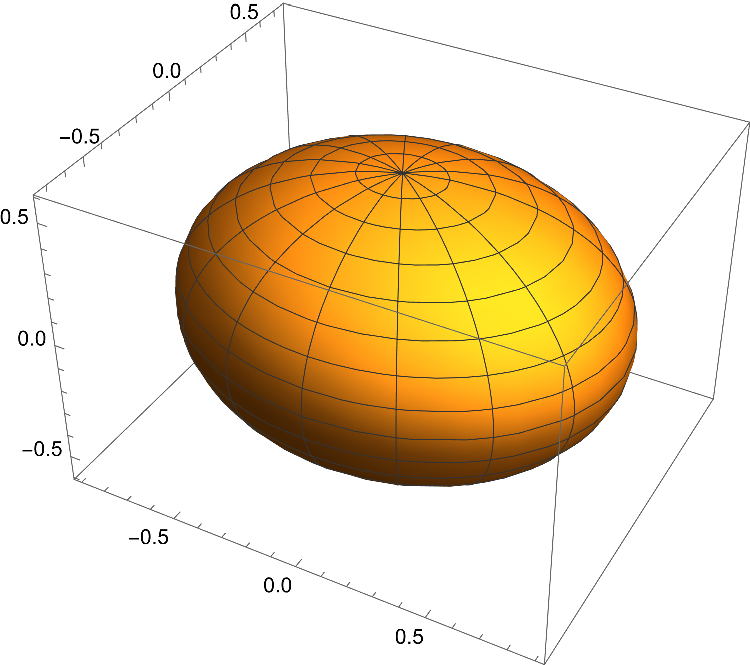
\includegraphics[width=\linewidth]{figures/tuoqiu.pdf}}
                         \end{minipage}  & $\dfrac{x^2}{a^2}+\dfrac{y^2}{b^2}+\dfrac{z^2}{c^2}=1$  & $\begin{cases}
                                                                                                              x=a\sin u\cos v \\y=\sin u\sin v\\z=c\cos u\\u\in[0,\pi],v\in[0,2\pi]
                                                                                                          \end{cases}$                              \\
            \midrule
            椭圆锥面   & \begin{minipage}[b]{0.3\columnwidth}
                             \raisebox{-.5\height}{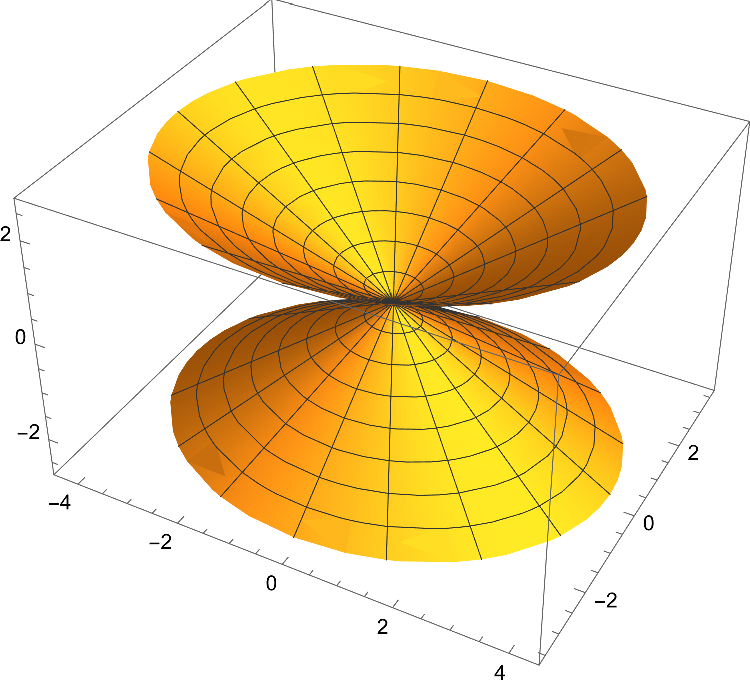
\includegraphics[width=\linewidth]{figures/tuoyuanzm.pdf}}
                         \end{minipage} & $\dfrac{x^2}{a^2}+\dfrac{y^2}{b^2}=z^2$                 & $\begin{cases}
                                                                                                             x=av\cos u \\y=bv\sin u\\z=cv\\u\in[0,2\pi],v\in\mathbb{R}
                                                                                                         \end{cases}$                                          \\
            \midrule
            椭圆抛物面 & \begin{minipage}[b]{0.3\columnwidth}
                             \raisebox{-.5\height}{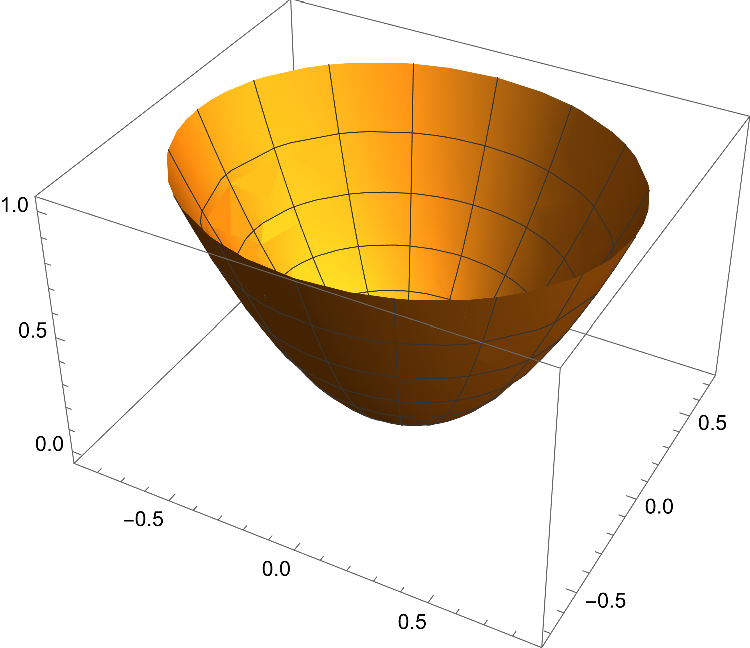
\includegraphics[width=\linewidth]{figures/tuoyuanpwm.pdf}}
                         \end{minipage} & $\dfrac{x^2}{a^2}+\dfrac{y^2}{b^2}=z$                   & $\begin{cases}
                                                                                                             x=av\cos u \\y=bv\sin u\\z=u^2\\u\in[0,2\pi],v\in[0,+\infty)
                                                                                                         \end{cases}$                                        \\
            \midrule
            双曲抛物面 & \begin{minipage}[b]{0.3\columnwidth}
                             \raisebox{-.5\height}{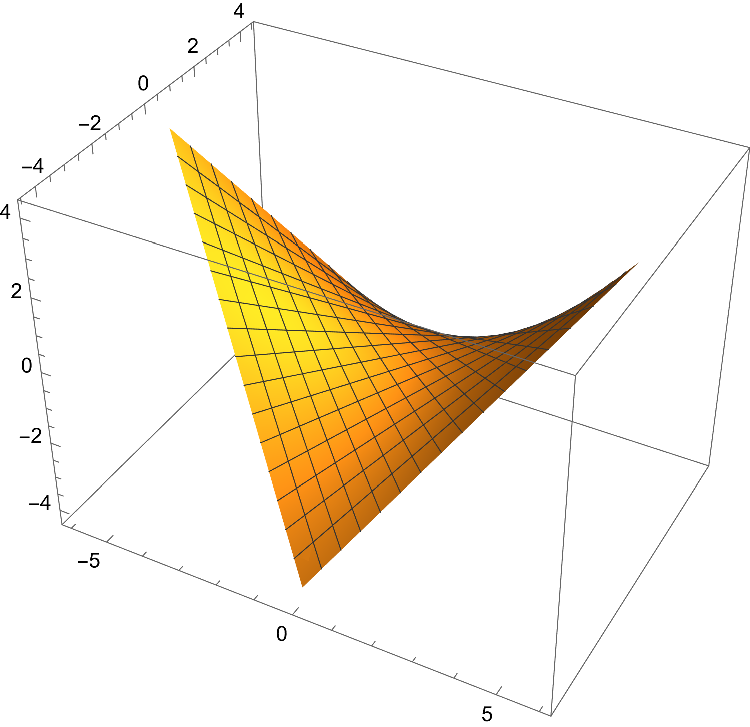
\includegraphics[width=\linewidth]{figures/shuangqpwm.pdf}}
                         \end{minipage} & $\dfrac{x^2}{a^2}-\dfrac{y^2}{b^2}=z$                   & $\begin{cases}
                                                                                                             x=a(u+v) \\y=b(u-v)\\z=4uv\\u,v\in\mathbb{R}
                                                                                                         \end{cases}$                                                        \\
            \midrule
            单叶双曲面 & \begin{minipage}[b]{0.3\columnwidth}
                             \raisebox{-.5\height}{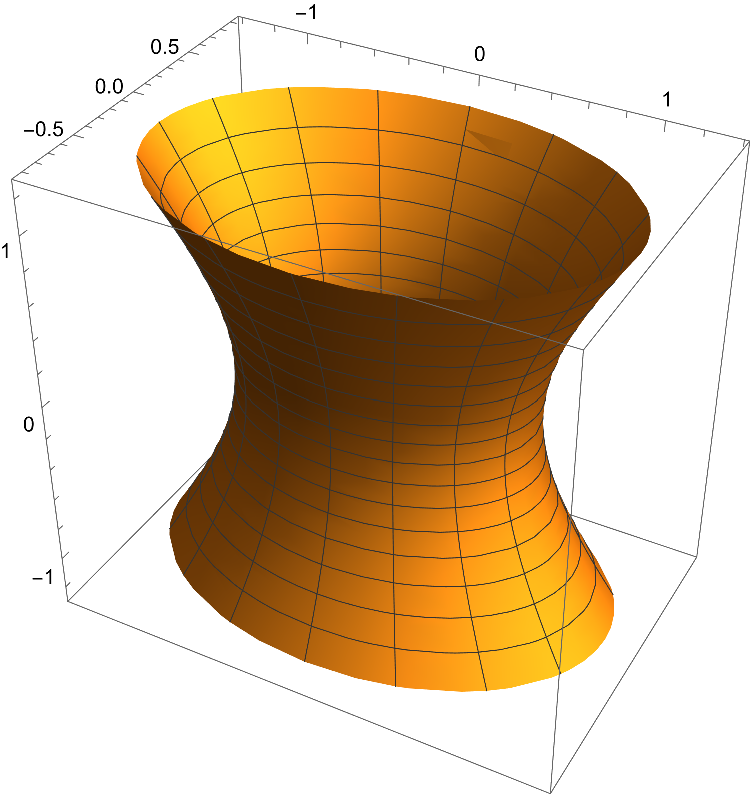
\includegraphics[width=\linewidth]{figures/danyesqm.pdf}}
                         \end{minipage} & $\dfrac{x^2}{a^2}+\dfrac{y^2}{b^2}-\dfrac{z^2}{c^2}=1$  & $\begin{cases}
                                                                                                             x=a\cosh u\cos v \\y=b\cosh u\sin v\\z=c\sinh u\\u\in\mathbb{R},v\in[0,2\pi]\\
                                                                                                         \end{cases}$                        \\
            \midrule
            双叶双曲面 & \begin{minipage}[b]{0.3\columnwidth}
                             \raisebox{-.5\height}{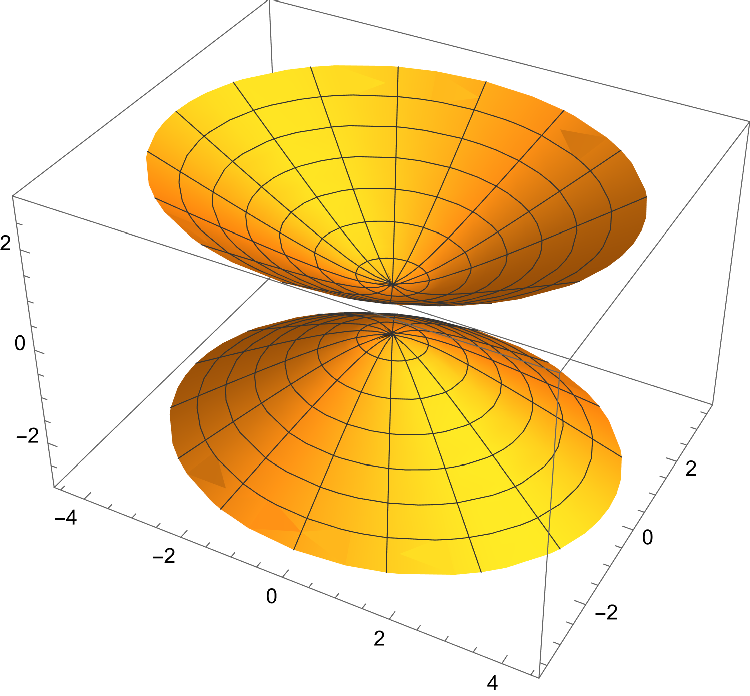
\includegraphics[width=\linewidth]{figures/shuangyesqm.pdf}}
                         \end{minipage} & $\dfrac{x^2}{a^2}+\dfrac{y^2}{b^2}-\dfrac{z^2}{c^2}=-1$ & $\begin{cases}
                                                                                                             x=a\sqrt{u^2-1}\cos v \\y=b\sqrt{u^2-1}\sin v\\z=cu\\u\in(-\infty,-1]\cup[1,+\infty),v\in\mathbb{R}
                                                                                                         \end{cases}$
        \end{tabular}
    }
\end{table}

\subsection{空间曲线及其方程}

\subsubsection{常见的曲线及其对应方程}

% \paragraph{摆线}

摆线是一种具有特定形状的曲线, 也被称为牛顿螺线或纽曼线.
它是由一个固定点上的一根线不断转动而形成的曲线, 其特点是曲线上的每个点到固定点的距离与该点在曲线上的位置成正比.

\begin{figure}[H]
    \centering
    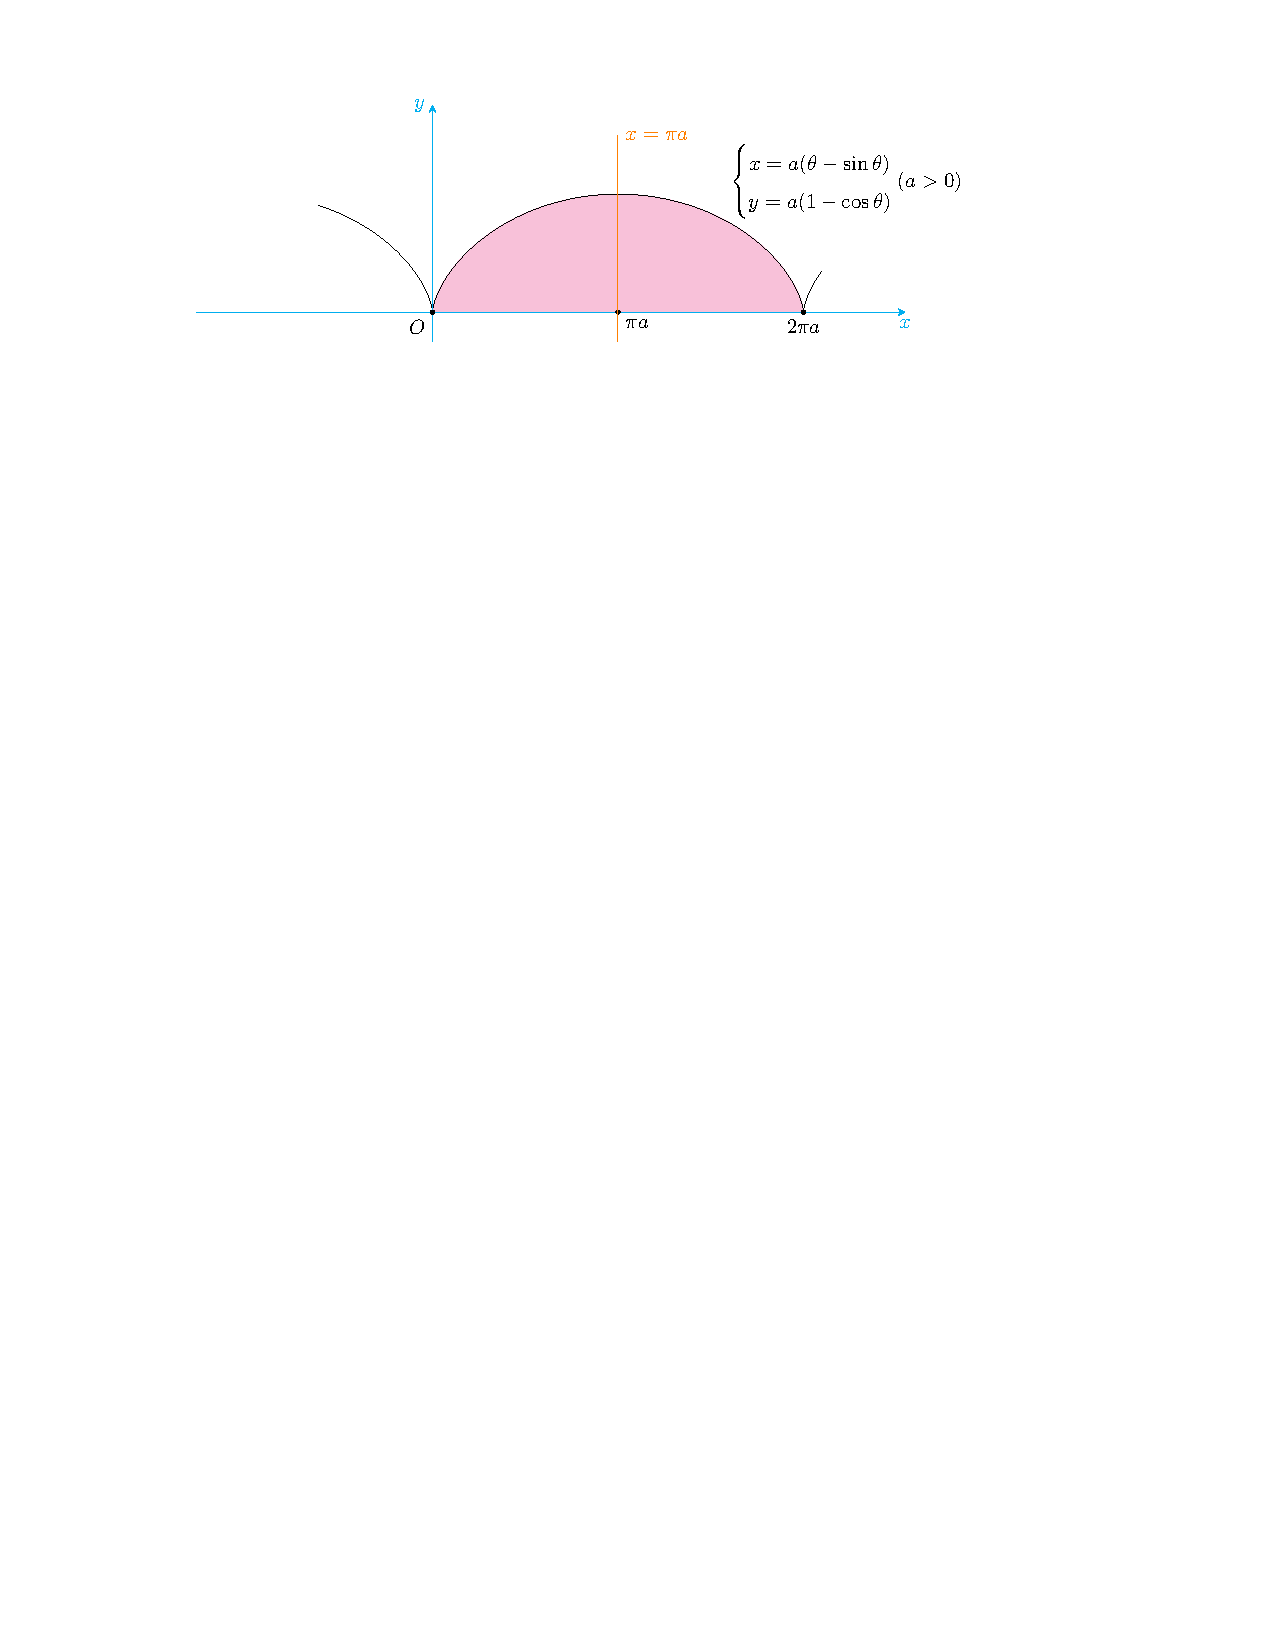
\includegraphics{figures/Cycloid.pdf}
    \caption{摆线}
    \label{cycloid}
\end{figure}

\begin{example}
    设摆线 $\begin{cases}
            x=a(t-\sin t) \\ y=a(1-\cos t)
        \end{cases}(0\leqslant t\leqslant 2\pi, a>0)$, 与 $x$ 轴所围平面图形为 $D$, 求 $D$ 分别绕 $x$ 轴, $y$ 轴以及绕 $y=2a$ 旋转一周所得旋转体的体积.
\end{example}
\begin{solution}
    由旋转体体积公式,
    \begin{flalign*}
        V_x    & =\pi\int_{0}^{2\pi a} f^2(x) \dd x=\pi \int_{0}^{2\pi} a^2(1-\cos t)^2 \dd (a(t-\sin t))=8\pi a^3\int_{0}^{2\pi} \sin^6\dfrac{t}{2} \dd t=32\pi a^3\int_{0}^{\frac{\pi}{2}} \sin^6t \dd t=5\pi^2a^3 \\
        V_y    & =2\pi\int_{0}^{2\pi a} xf(x) \dd x=2\pi a^3\int_{0}^{2\pi} (t-\sin t)(1-\cos t)^2 \dd t=2\pi a^3\cdot \qty(2\pi^2+\pi^2)=6\pi^3a^3                                                                  \\
        V_{2a} & =\pi (2a)^2\cdot 2\pi a-\pi \int_{0}^{2\pi a}(2a-y)^2\dd x=8\pi^2a^3-\pi a^3\int_{0}^{2\pi}\qty(1+\cos t-\cos^2t-\cos^3t)\dd t=7\pi ^2 a^3.
    \end{flalign*}
\end{solution}

% \paragraph{箕舌线}

箕舌线在数学中常用于曲线绘制和几何分析, 具有一定的研究和应用价值. 它的特殊形状和几何性质使其在数学教学和研究中具有一定的重要性.

\begin{figure}[H]
    \centering
    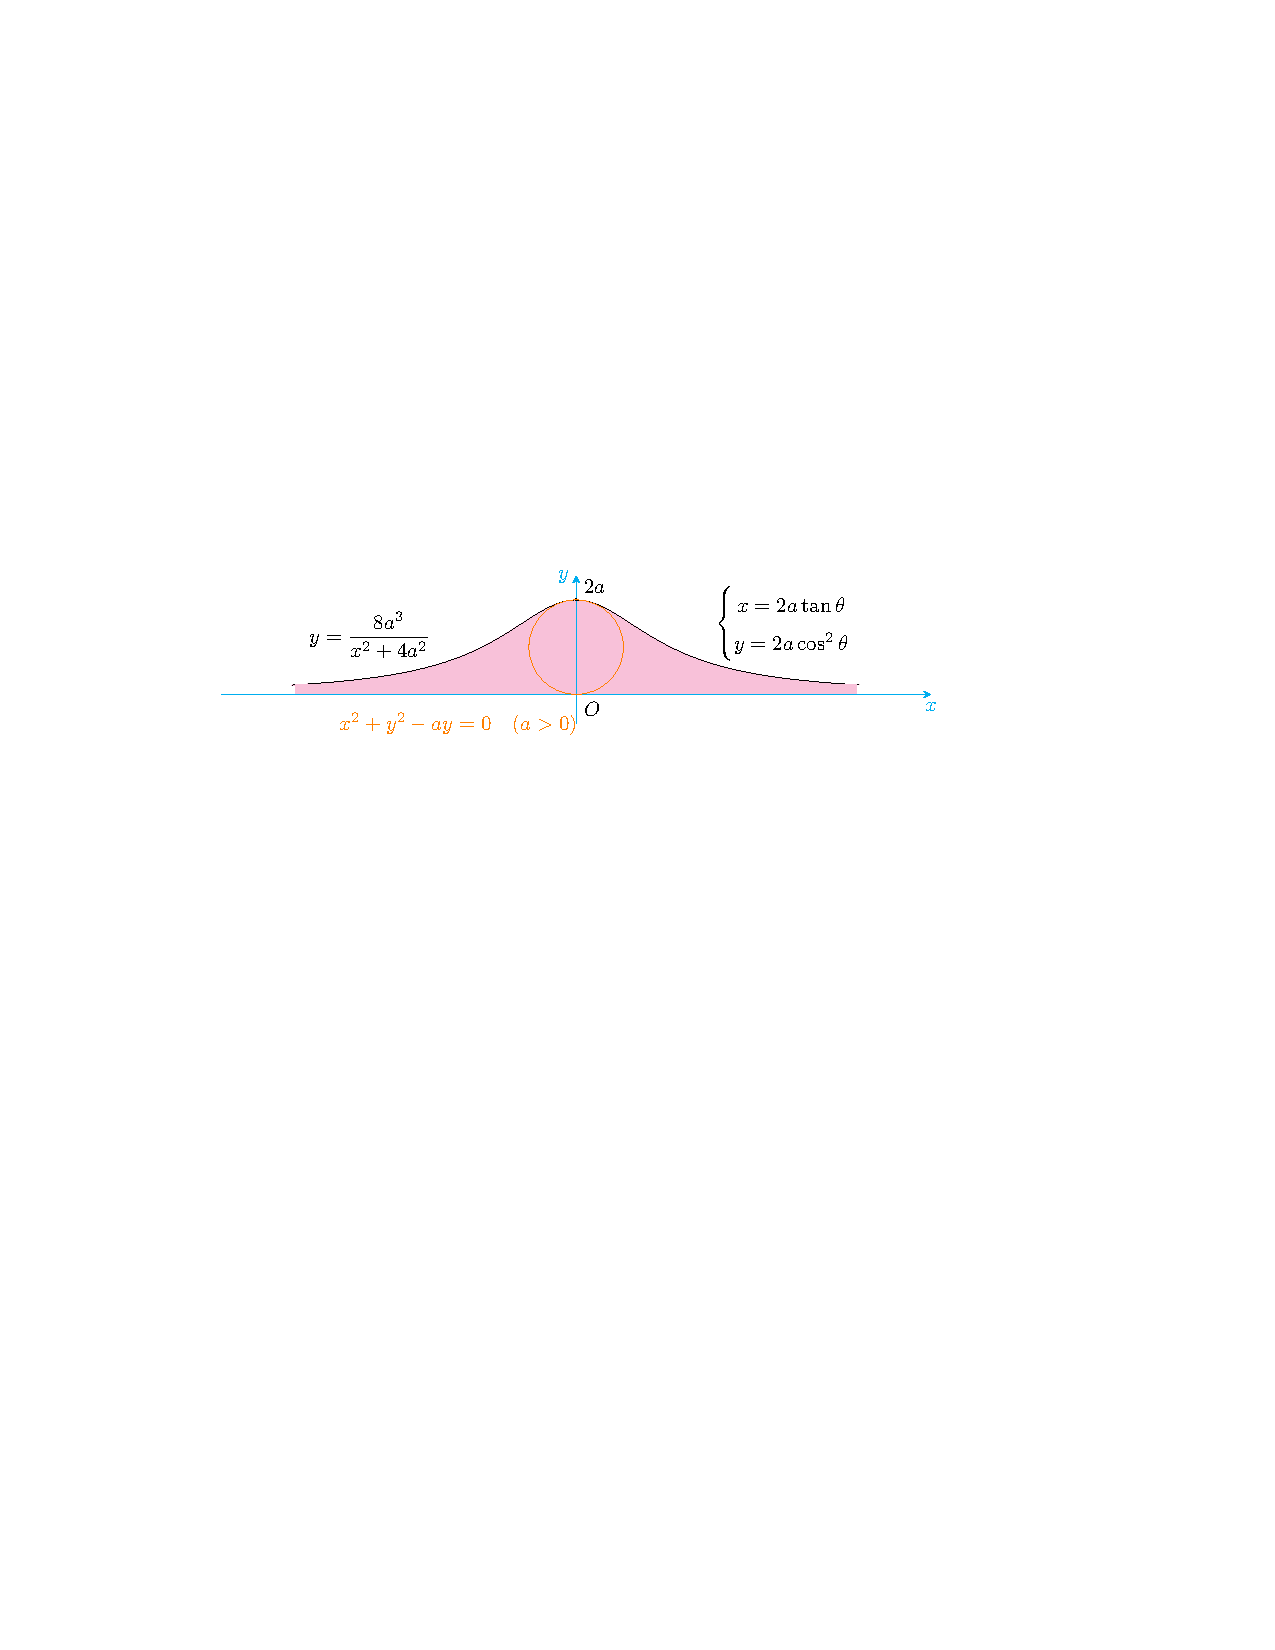
\includegraphics{figures/MiTongueLine.pdf}
    \caption{箕舌线}
    \label{miTongueLine}
\end{figure}

% \paragraph{双纽线}

双纽线是一种特殊的曲线形状, 也称为双纽结或双纽环. 它是一种具有对称性的闭合曲线, 形状类似于一个双环结构. 双纽线的数学表达式通常可以用参数方程或极坐标方程表示.

\begin{figure}[H]
    \centering
    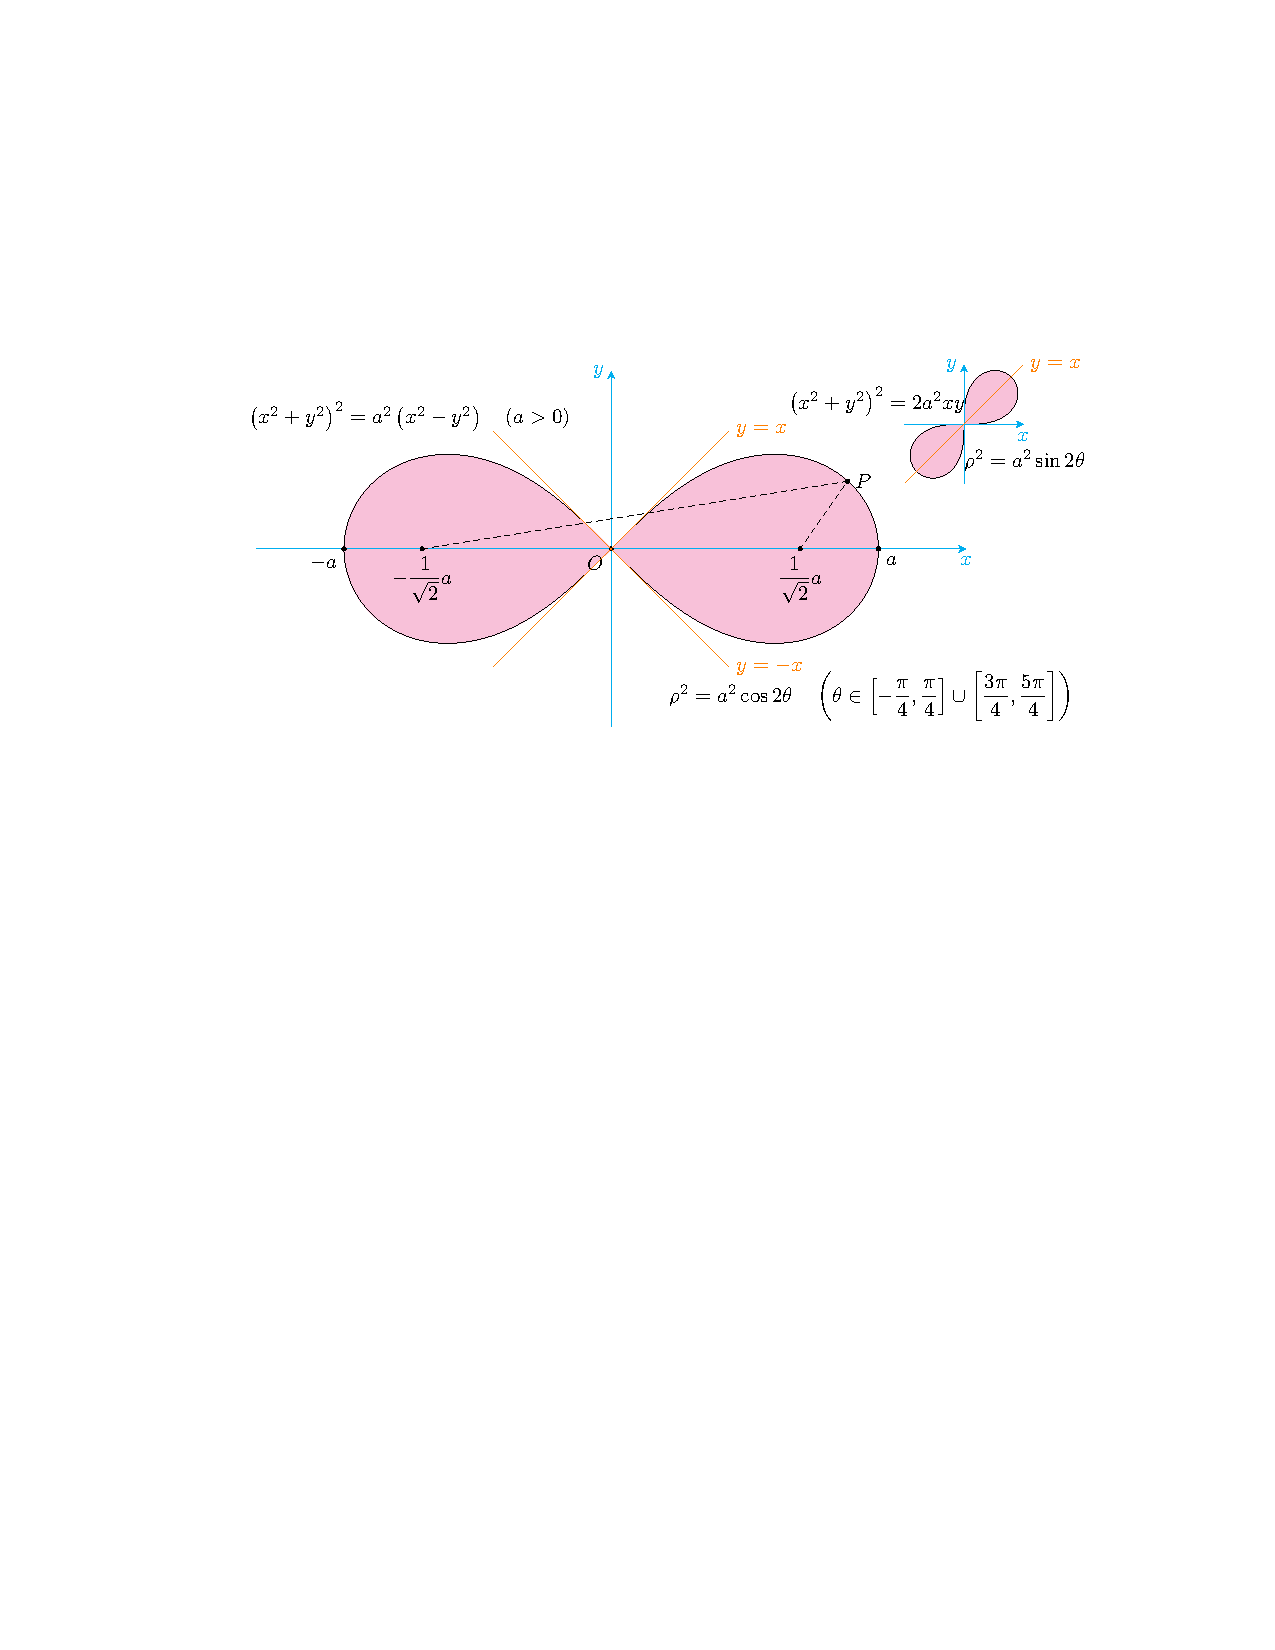
\includegraphics{figures/DoubleTwistedWire.pdf}
    \caption{双纽线}
    \label{doubleTwistedWire}
\end{figure}

\begin{example}
    计算双纽线 $\qty(x^2+y^2)^2=2a^2\qty(x^2-y^2)~(a>0)$ 的面积.
\end{example}
\begin{solution}
    由题意可得双纽线的极坐标方程为 $r^2=2a^2\cos 2\theta$, 且由对称性知
    $$
        S=4\times \dfrac{1}{2}\int_{0}^{\frac{\pi}{4}} 2a^2\cos 2\theta \dd \theta=4a^2\int_{0}^{\frac{\pi}{4}} \cos2\theta \dd \theta=2a^2.
    $$
\end{solution}

% \paragraph{对数螺线}

对数螺线是一种特殊的曲线形状, 也称为对数螺旋线或阿基米德螺线.

\begin{figure}[H]
    \centering
    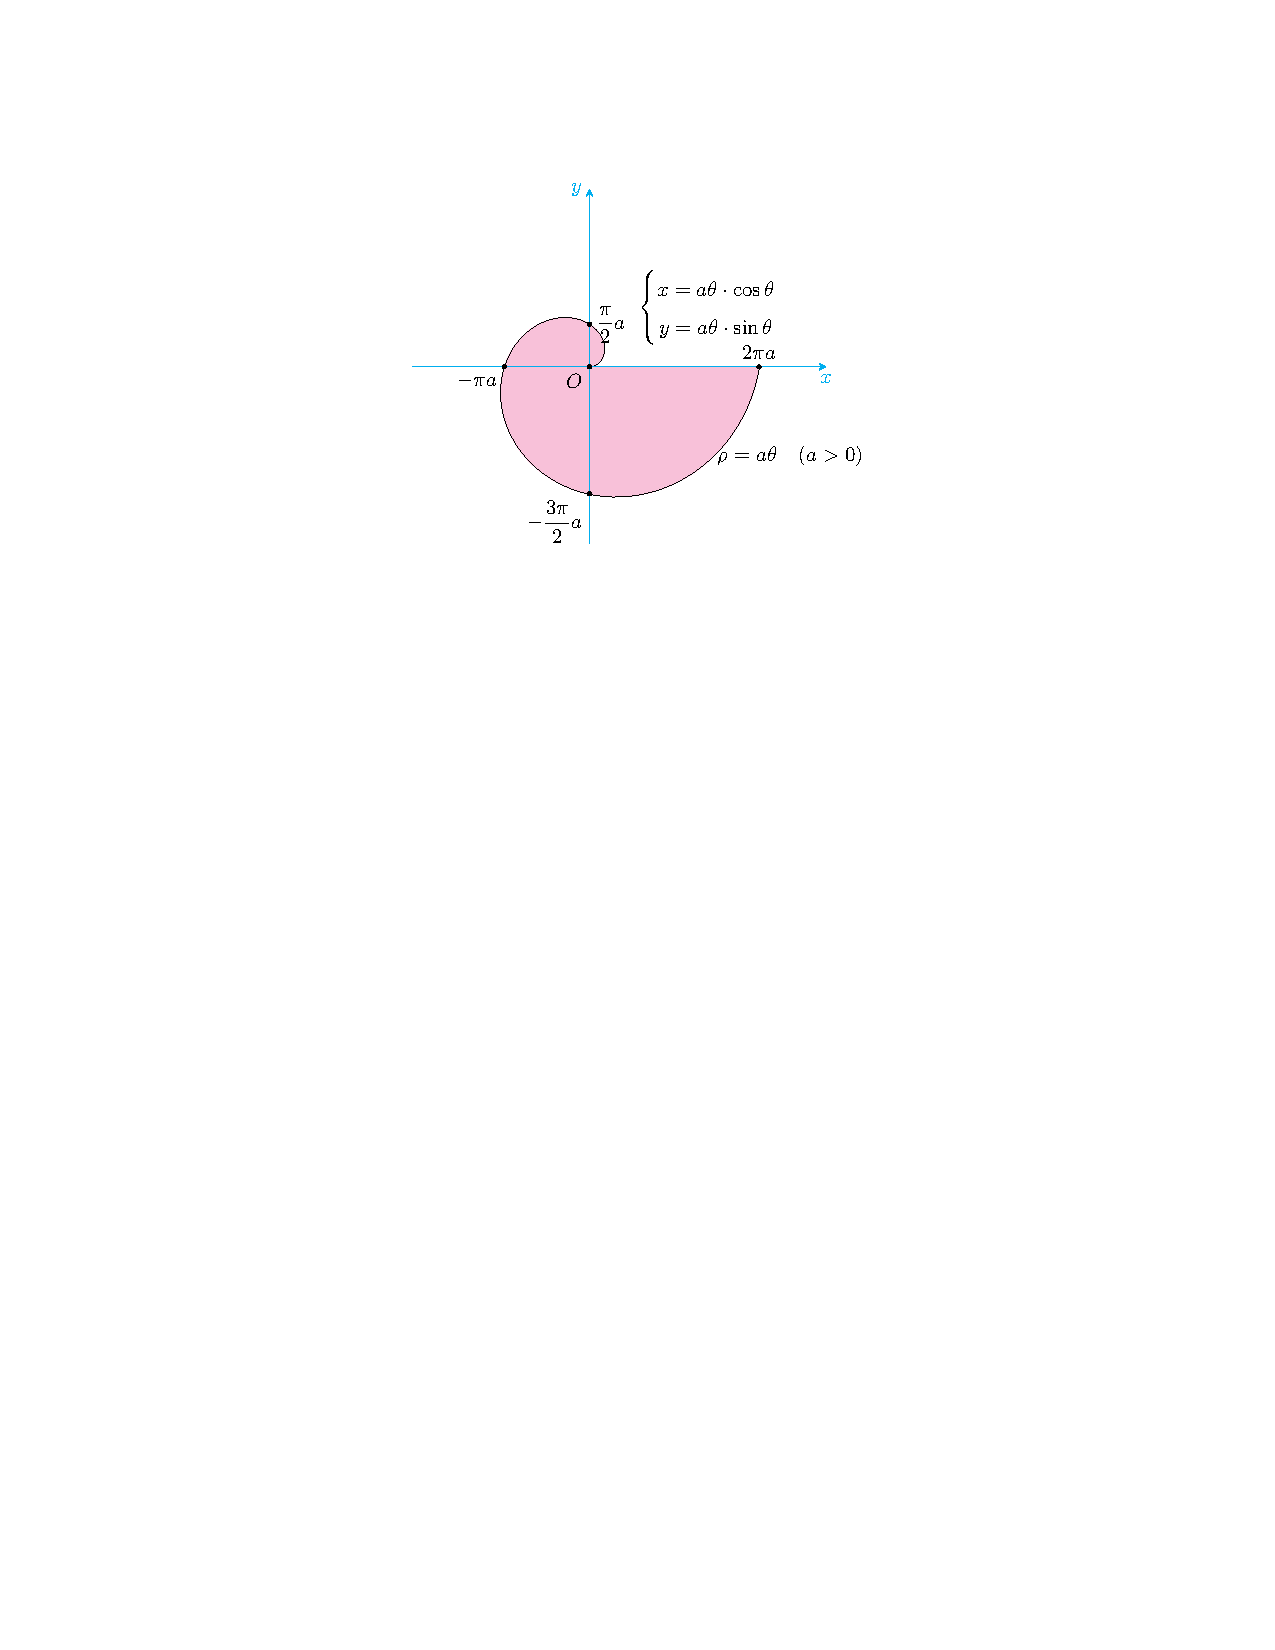
\includegraphics{figures/ArchimedesSpiral.pdf}
    \caption{对数螺线}
    \label{archimedesSpiral}
\end{figure}

% \paragraph{星形线}

在数学中, 星形线的定义比较宽泛, 可以包括多种形状. 例如, 五角星、六角星、七角星等都可以看作是一种星形线. 星形线的数学表达式可以有多种形式, 常见的包括极坐标方程、参数方程或直角坐标方程, 具体形式取决于所描述的具体星形线的形状和特征.

\begin{figure}[H]
    \centering
    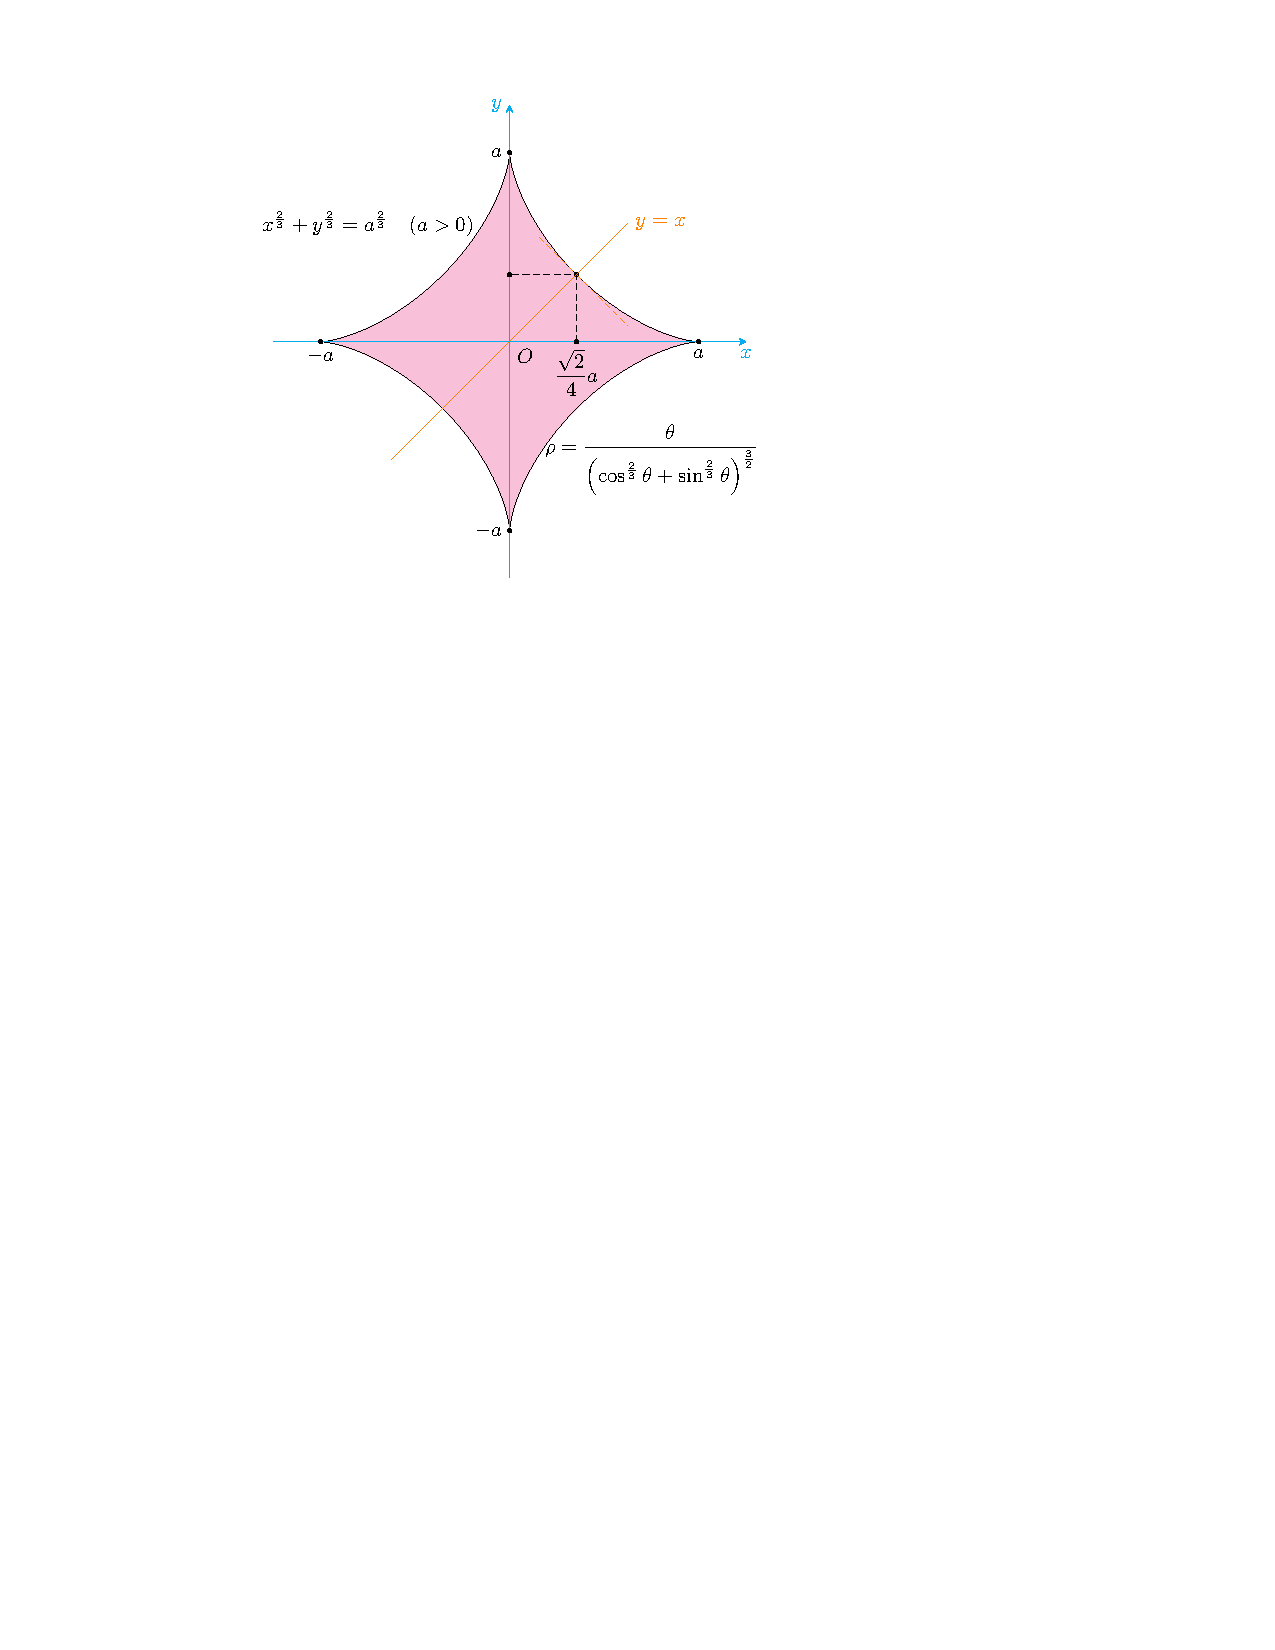
\includegraphics{figures/StarLine.pdf}
    \caption{星形线}
    \label{starLine}
\end{figure}

% \paragraph{心形线}

心形线是一种具有象征意义和浪漫情感的特殊曲线形状, 其外形类似于一个心形. 在数学上, 心形线可以用不同的数学表达式来描述, 常见的包括参数方程、极坐标方程或直角坐标方程.

\begin{figure}[H]
    \centering
    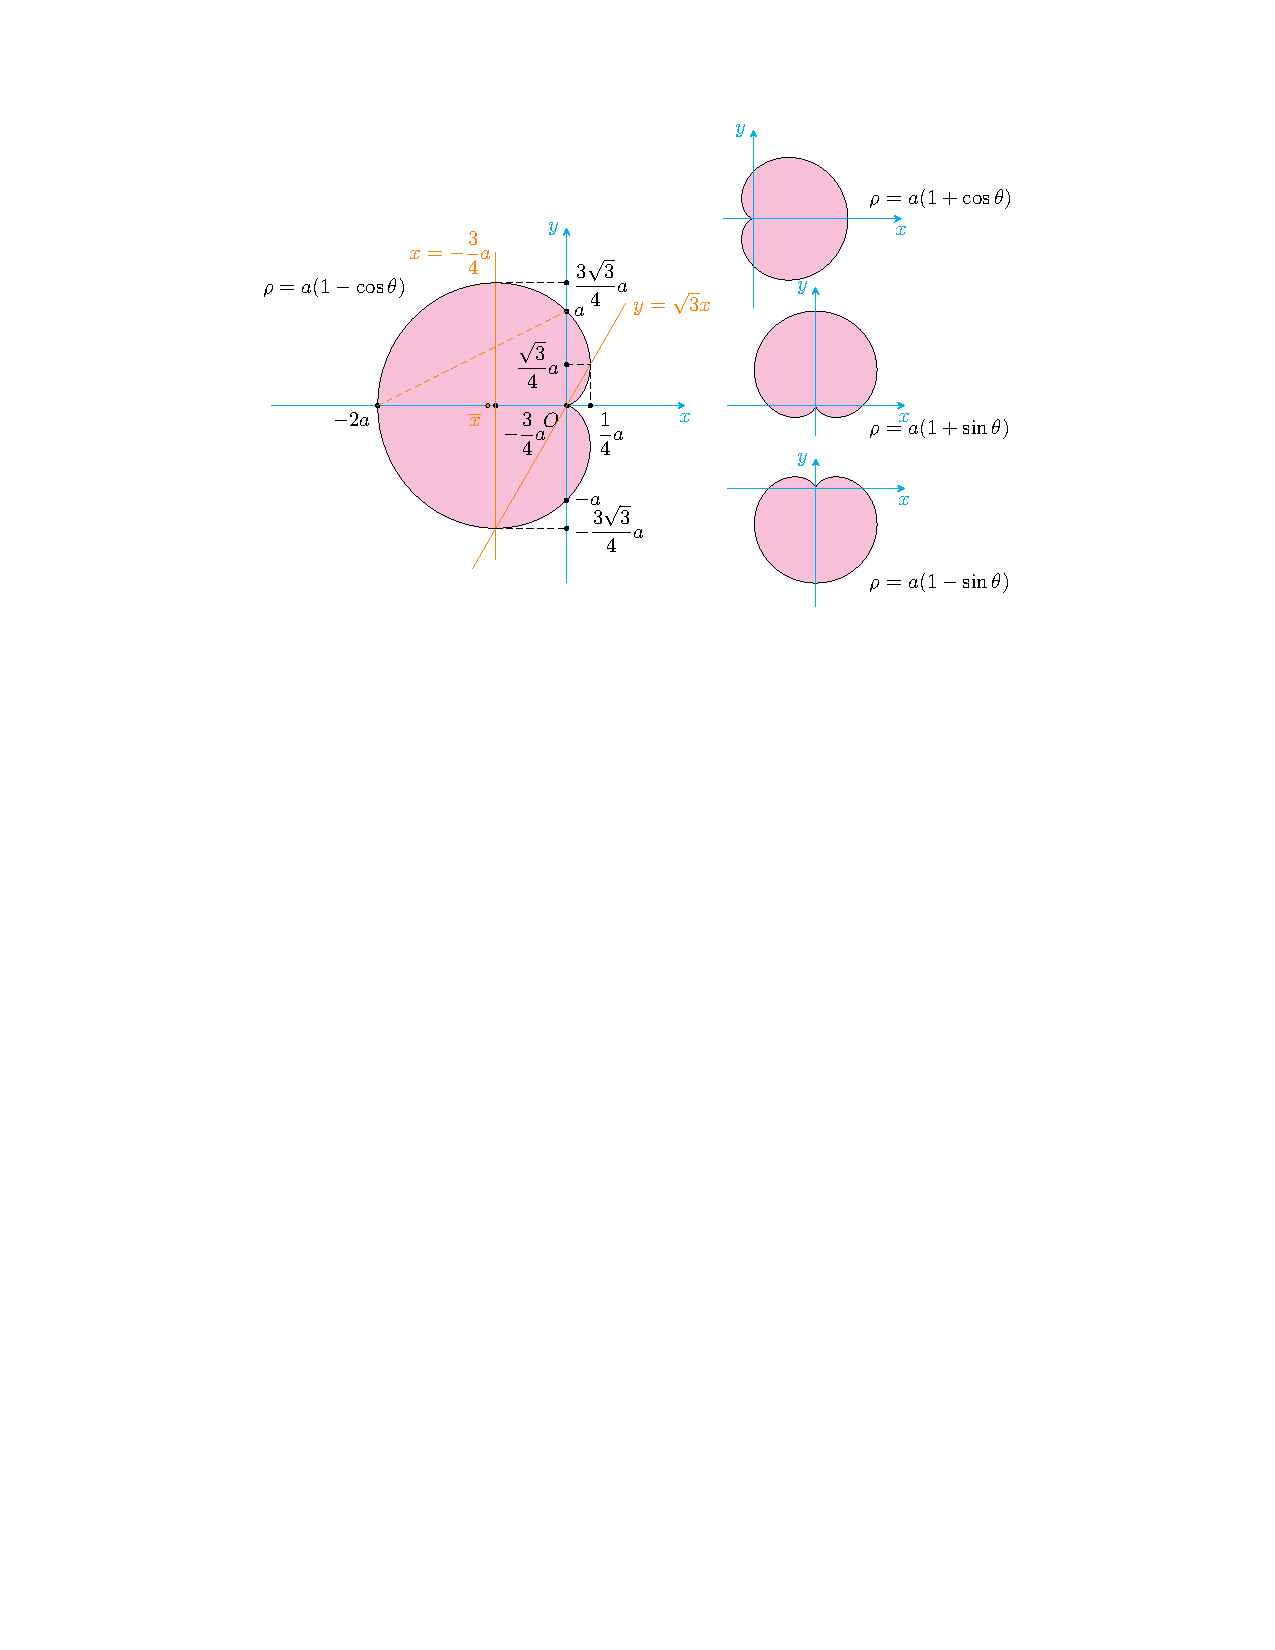
\includegraphics{figures/CardioidLine.pdf}
    \caption{心形线}
    \label{cardioidLine}
\end{figure}

\begin{example}
    计算心形线 $r=a(1+\cos\theta) ~(a>0)$ 的面积.
\end{example}
\begin{solution}
    由对称性知
    $$
        S=2\times\dfrac{1}{2}\int_{0}^{\pi} a^2(1+\cos\theta)^2 \dd \theta=\dfrac{3a^2}{2}\pi.
    $$
\end{solution}

% \paragraph{叶形线}

叶形线是一种特殊的曲线形状, 其轮廓类似于植物叶子的形状, 因此得名为叶形线. 在数学上, 叶形线可以用不同的数学表达式来描述, 常见的包括参数方程、极坐标方程或直角坐标方程.

\begin{figure}[H]
    \centering
    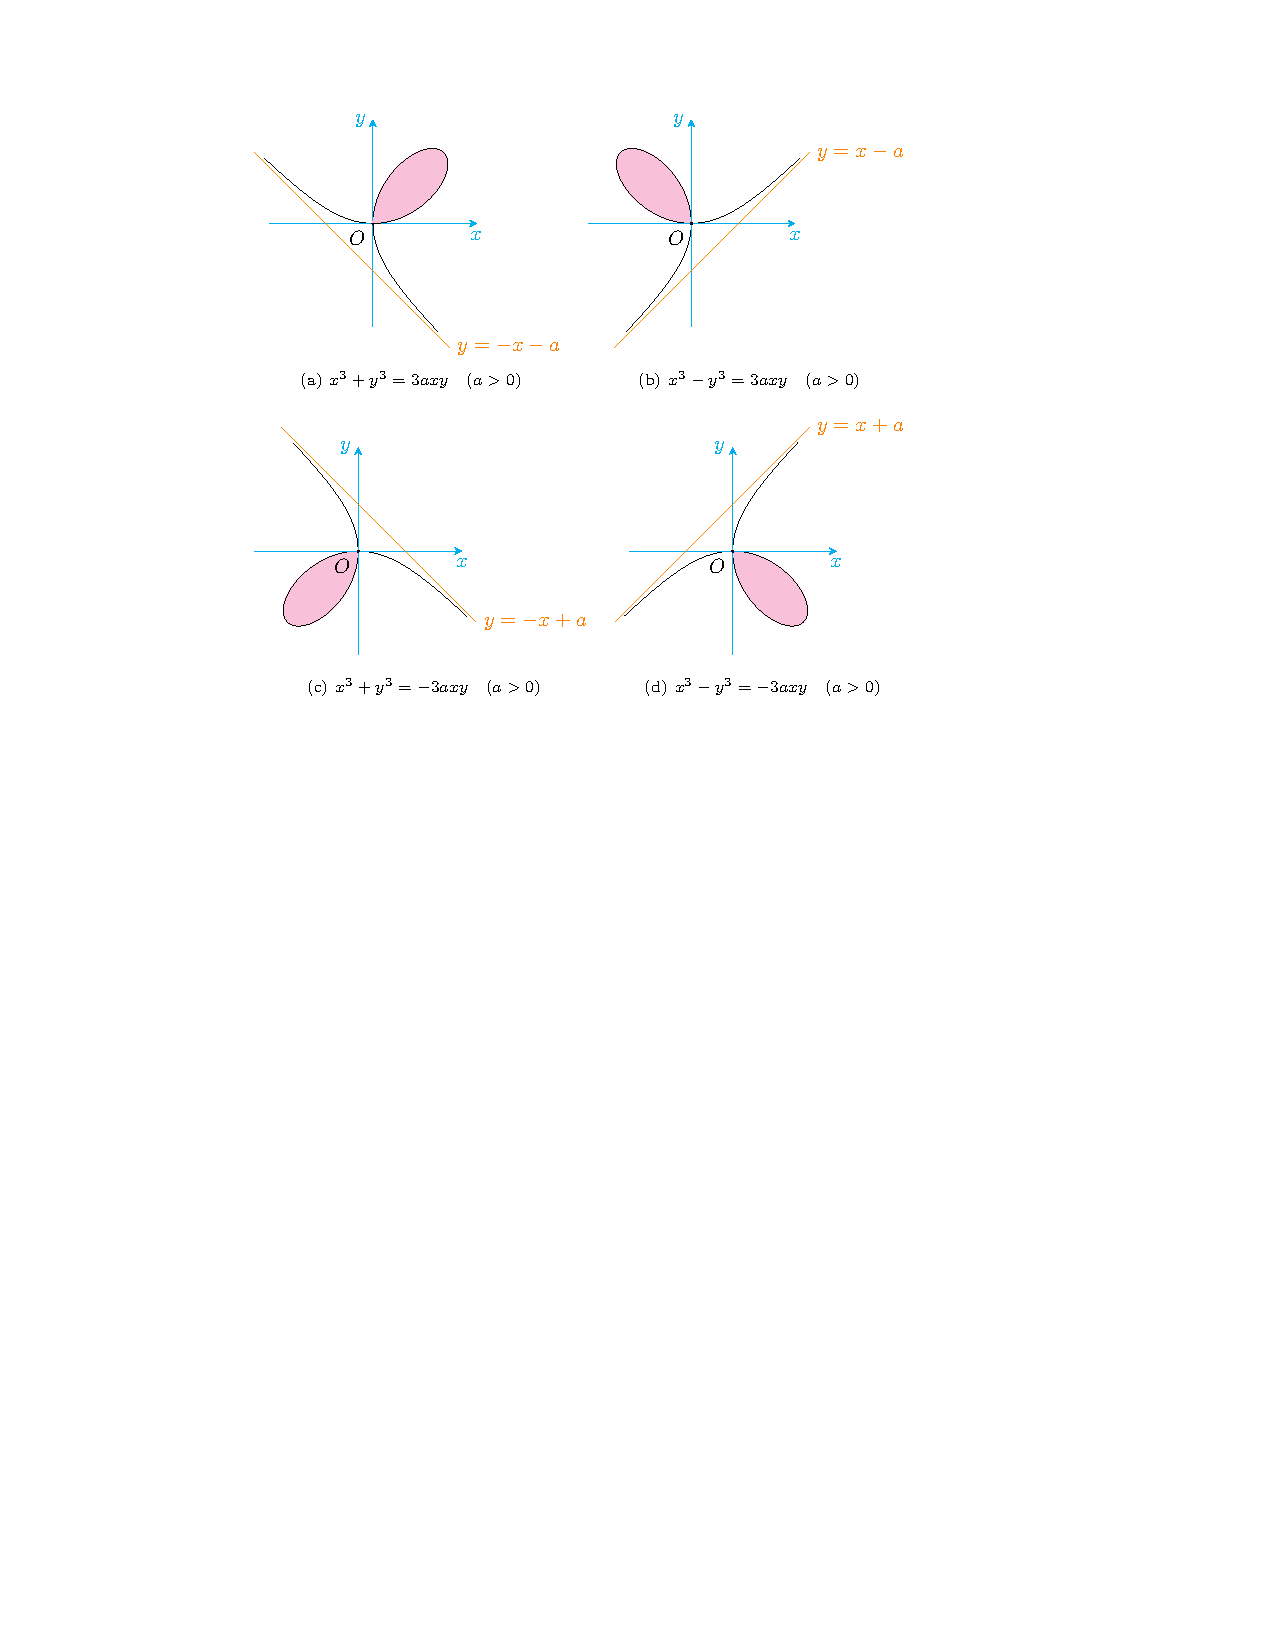
\includegraphics{figures/LeafLinear.pdf}
    \caption{叶形线}
    \label{leafLinear}
\end{figure}

% \paragraph{玫瑰线}

玫瑰线是一种经典的数学曲线, 其形状类似于玫瑰花的花瓣. 玫瑰线的美妙之处在于其优美的几何形状和对称性, 不同的 $n$ 值可以得到不同朵花瓣的玫瑰线, 每一朵花瓣都充满了艺术感和美感.

\begin{figure}[H]
    \centering
    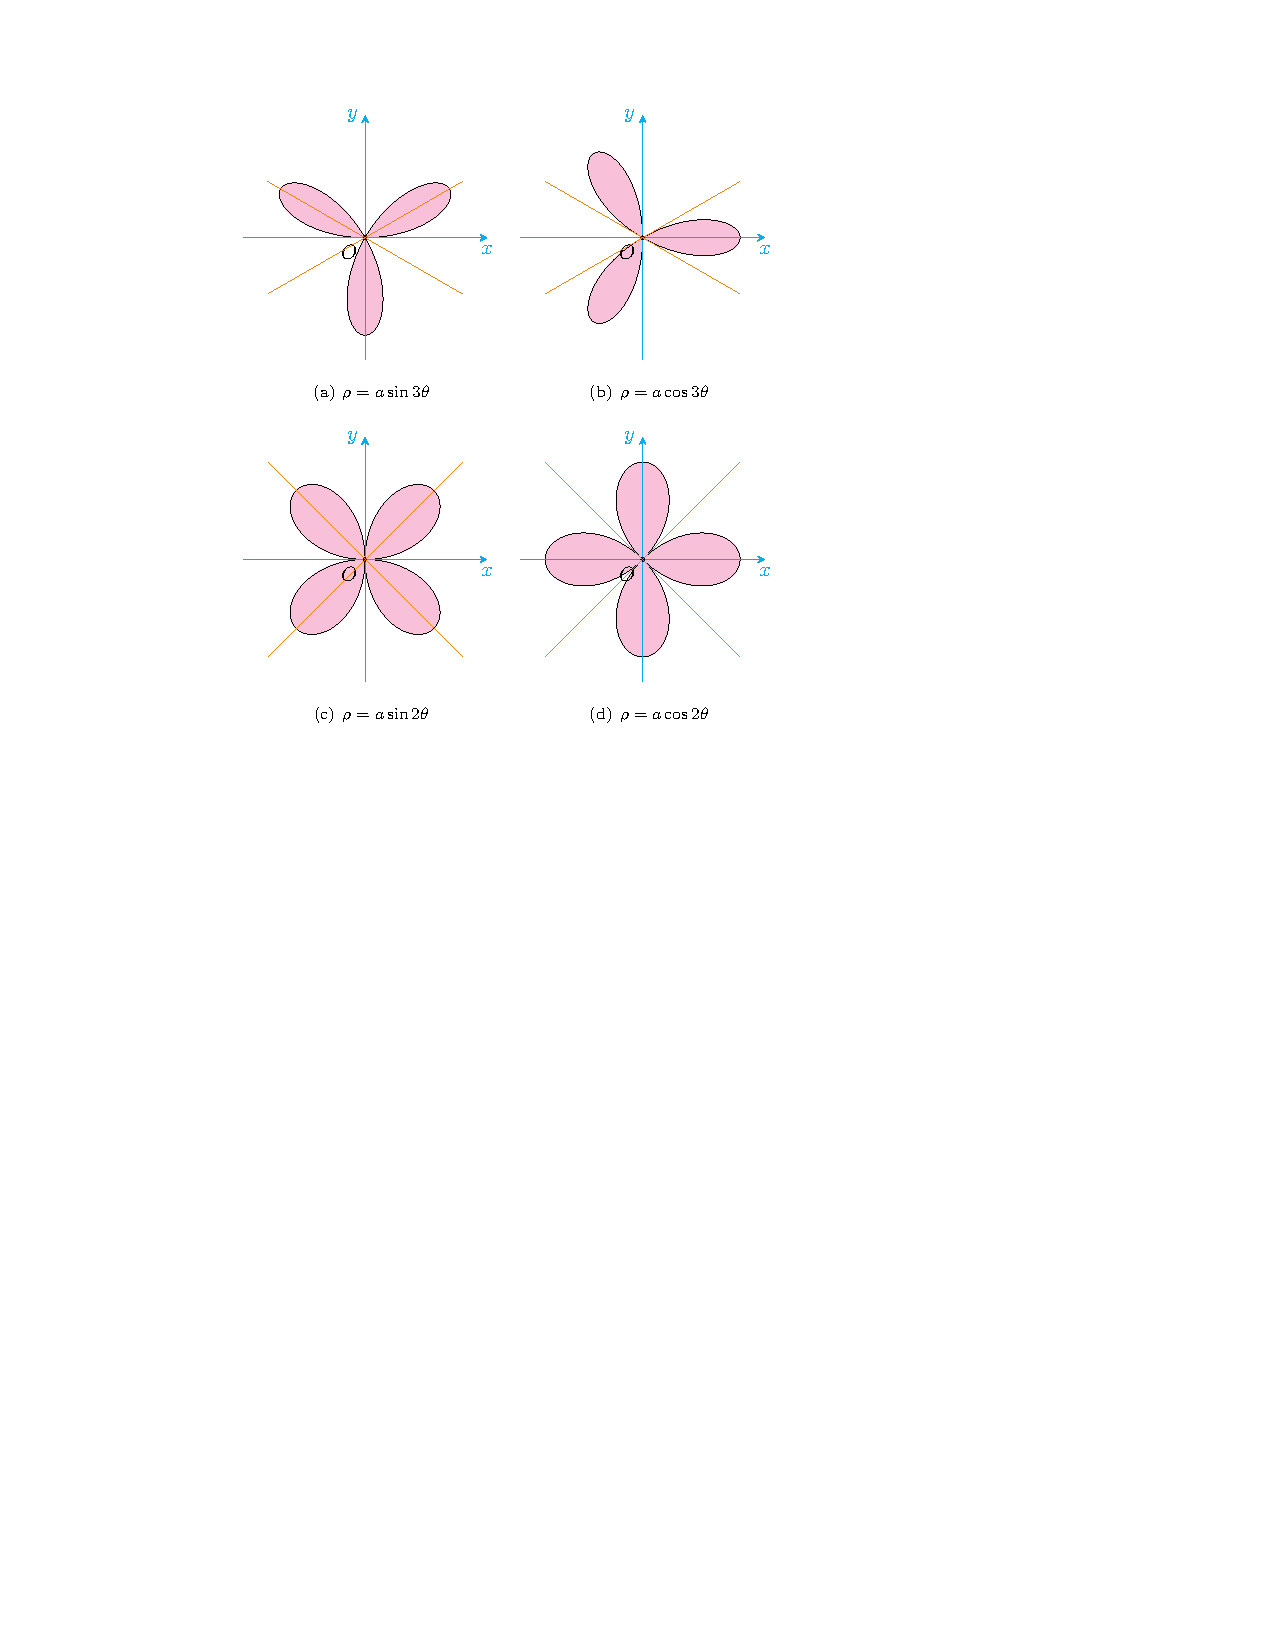
\includegraphics{figures/RoseLine.pdf}
    \caption{玫瑰线}
    \label{roseLine}
\end{figure}

% \begin{figure}[H]
%     \centering
%     \subfigure[摆线]{
%         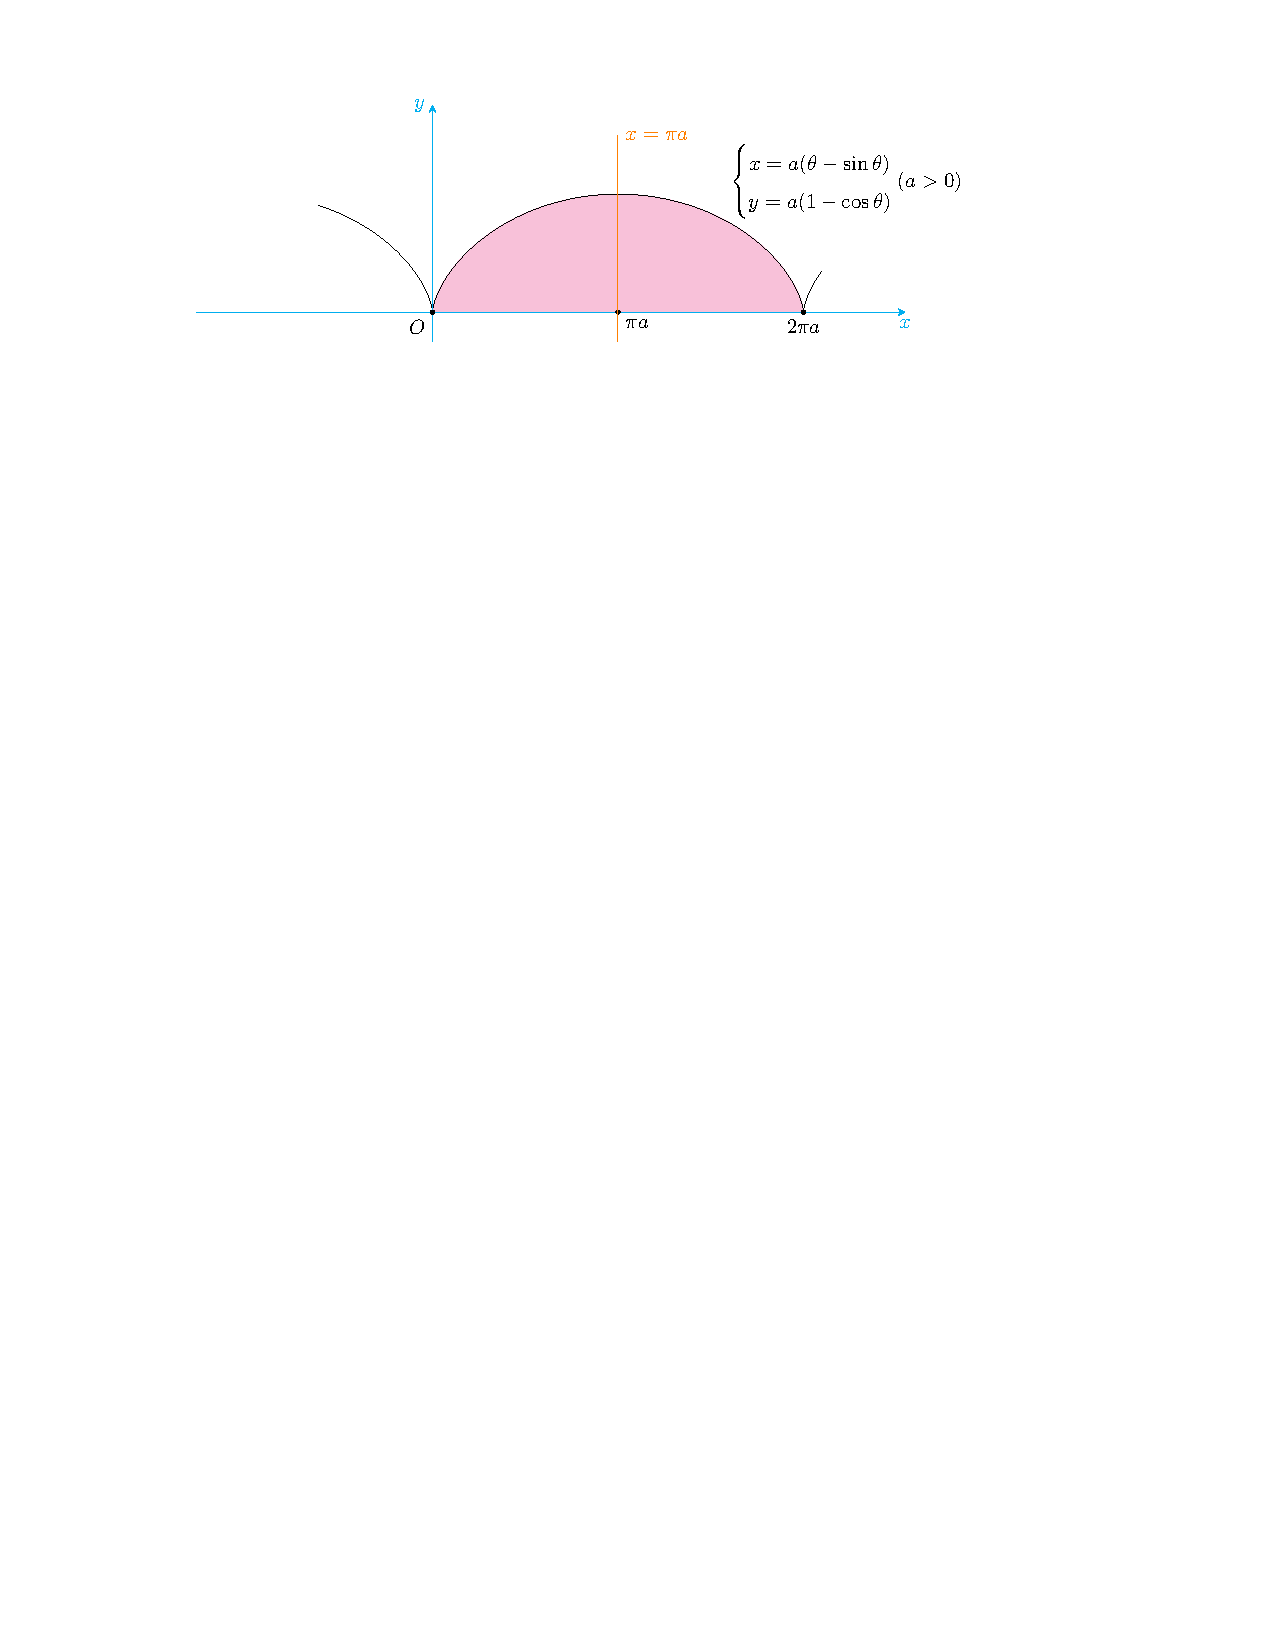
\includegraphics[scale=0.5]{figures/Cycloid.pdf}
%     }
%     \subfigure[箕舌线]{
%         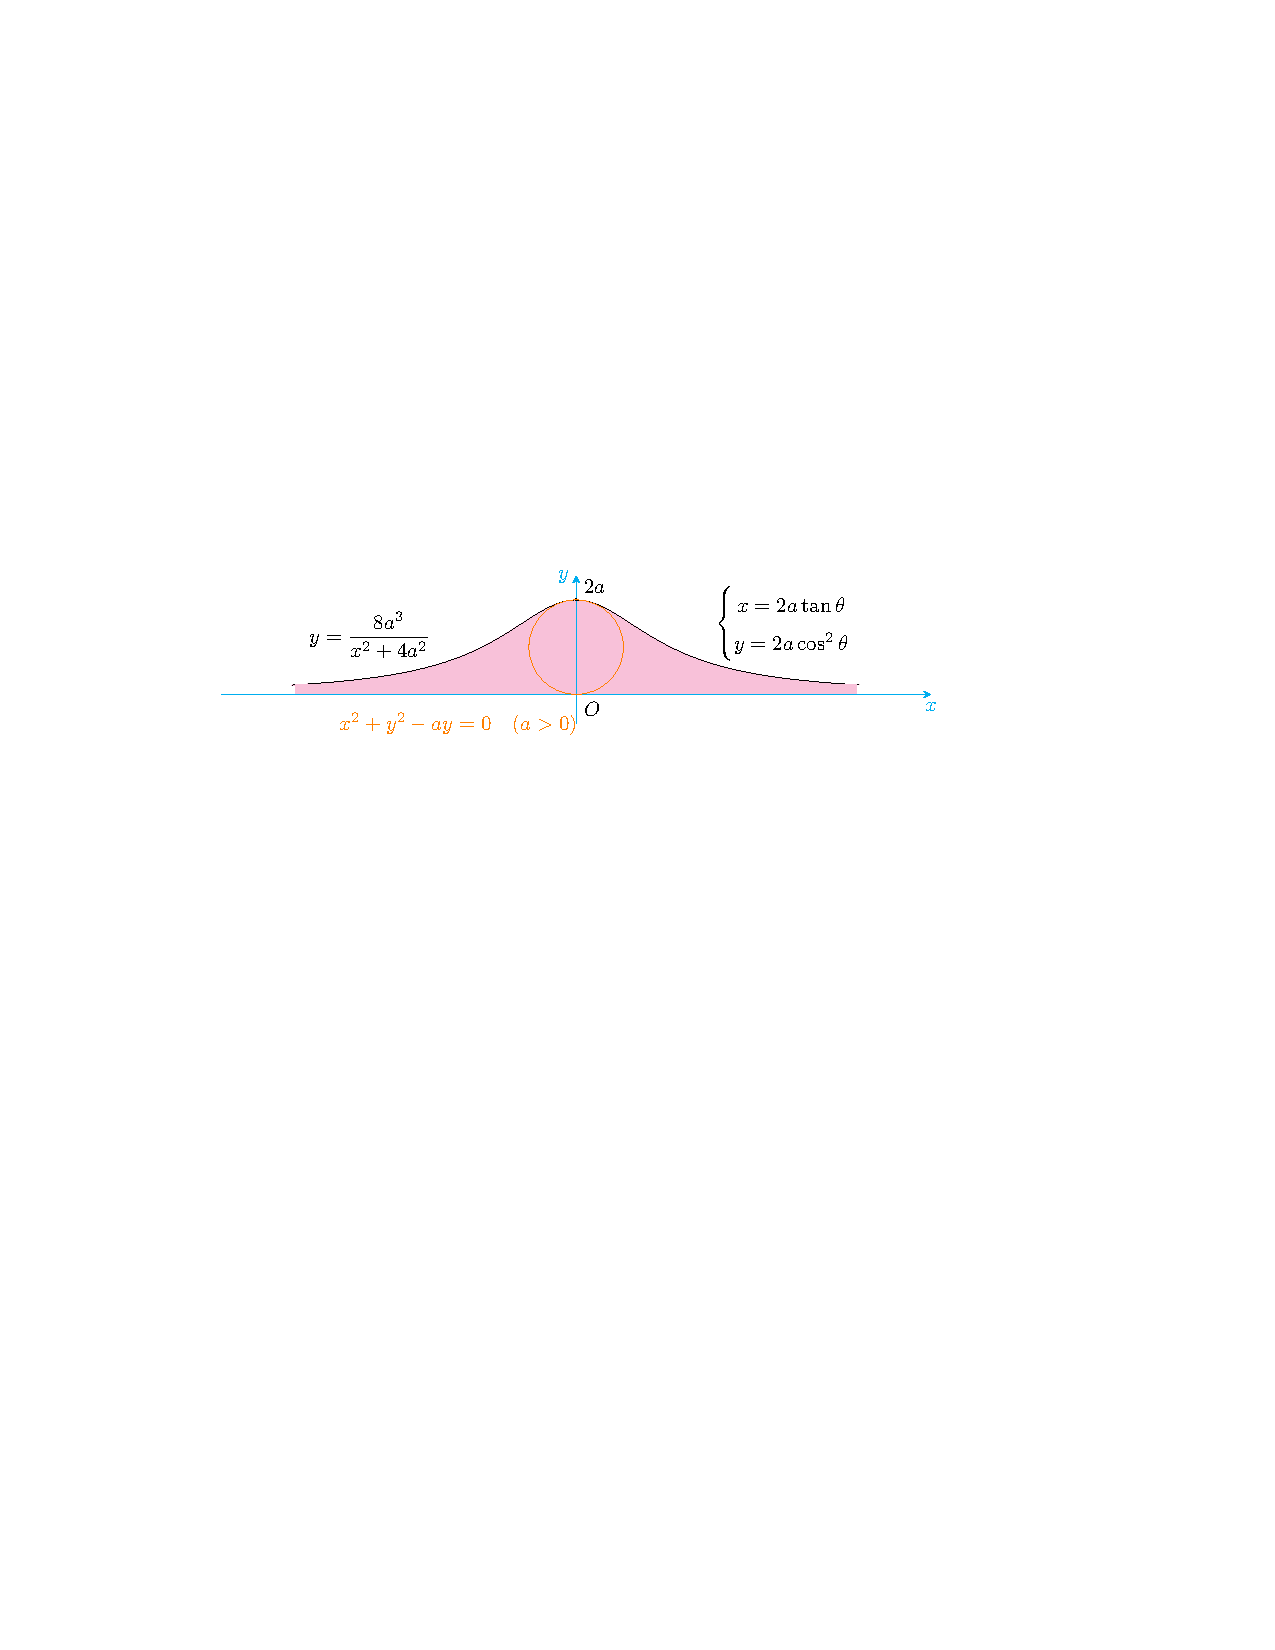
\includegraphics[scale=0.5]{figures/MiTongueLine.pdf}
%     }\\
%     \subfigure[双纽线]{
%         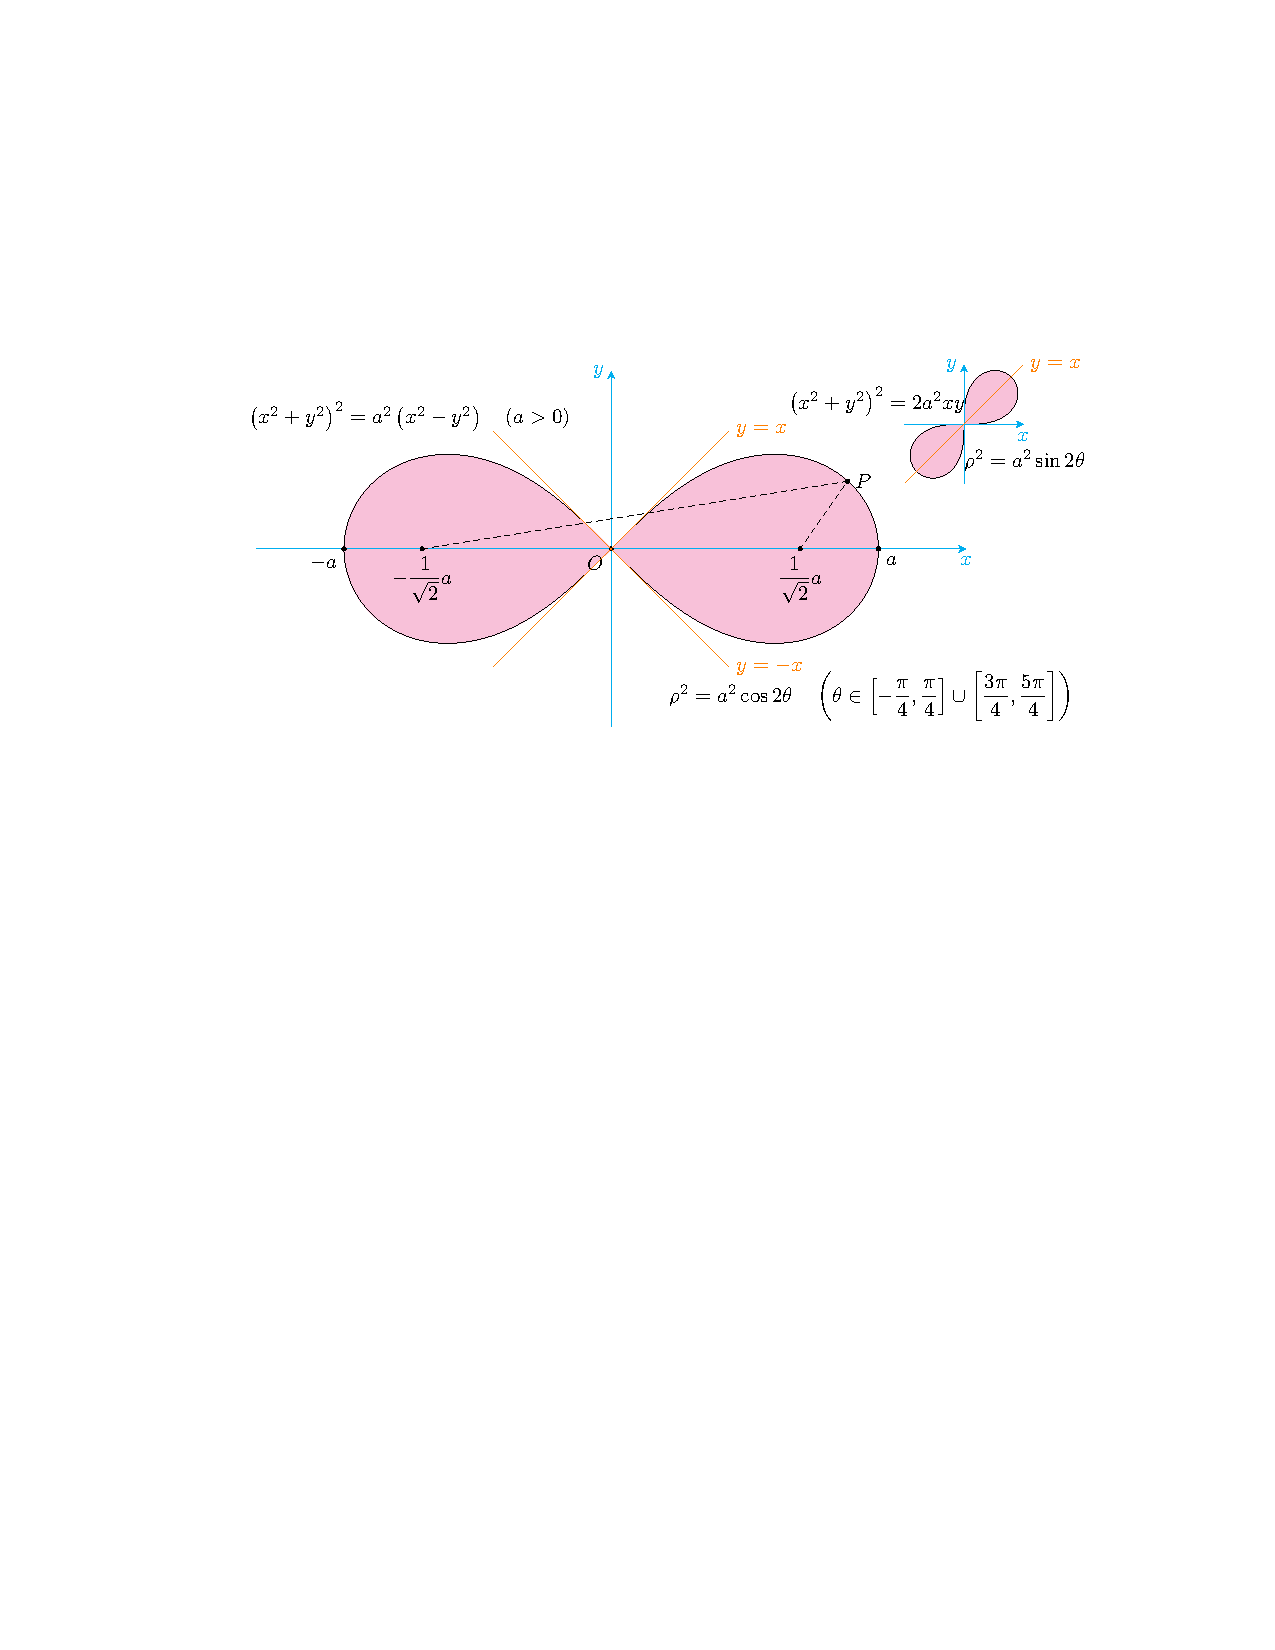
\includegraphics[scale=0.5]{figures/DoubleTwistedWire.pdf}
%     }
%     \subfigure[对数螺线]{
%         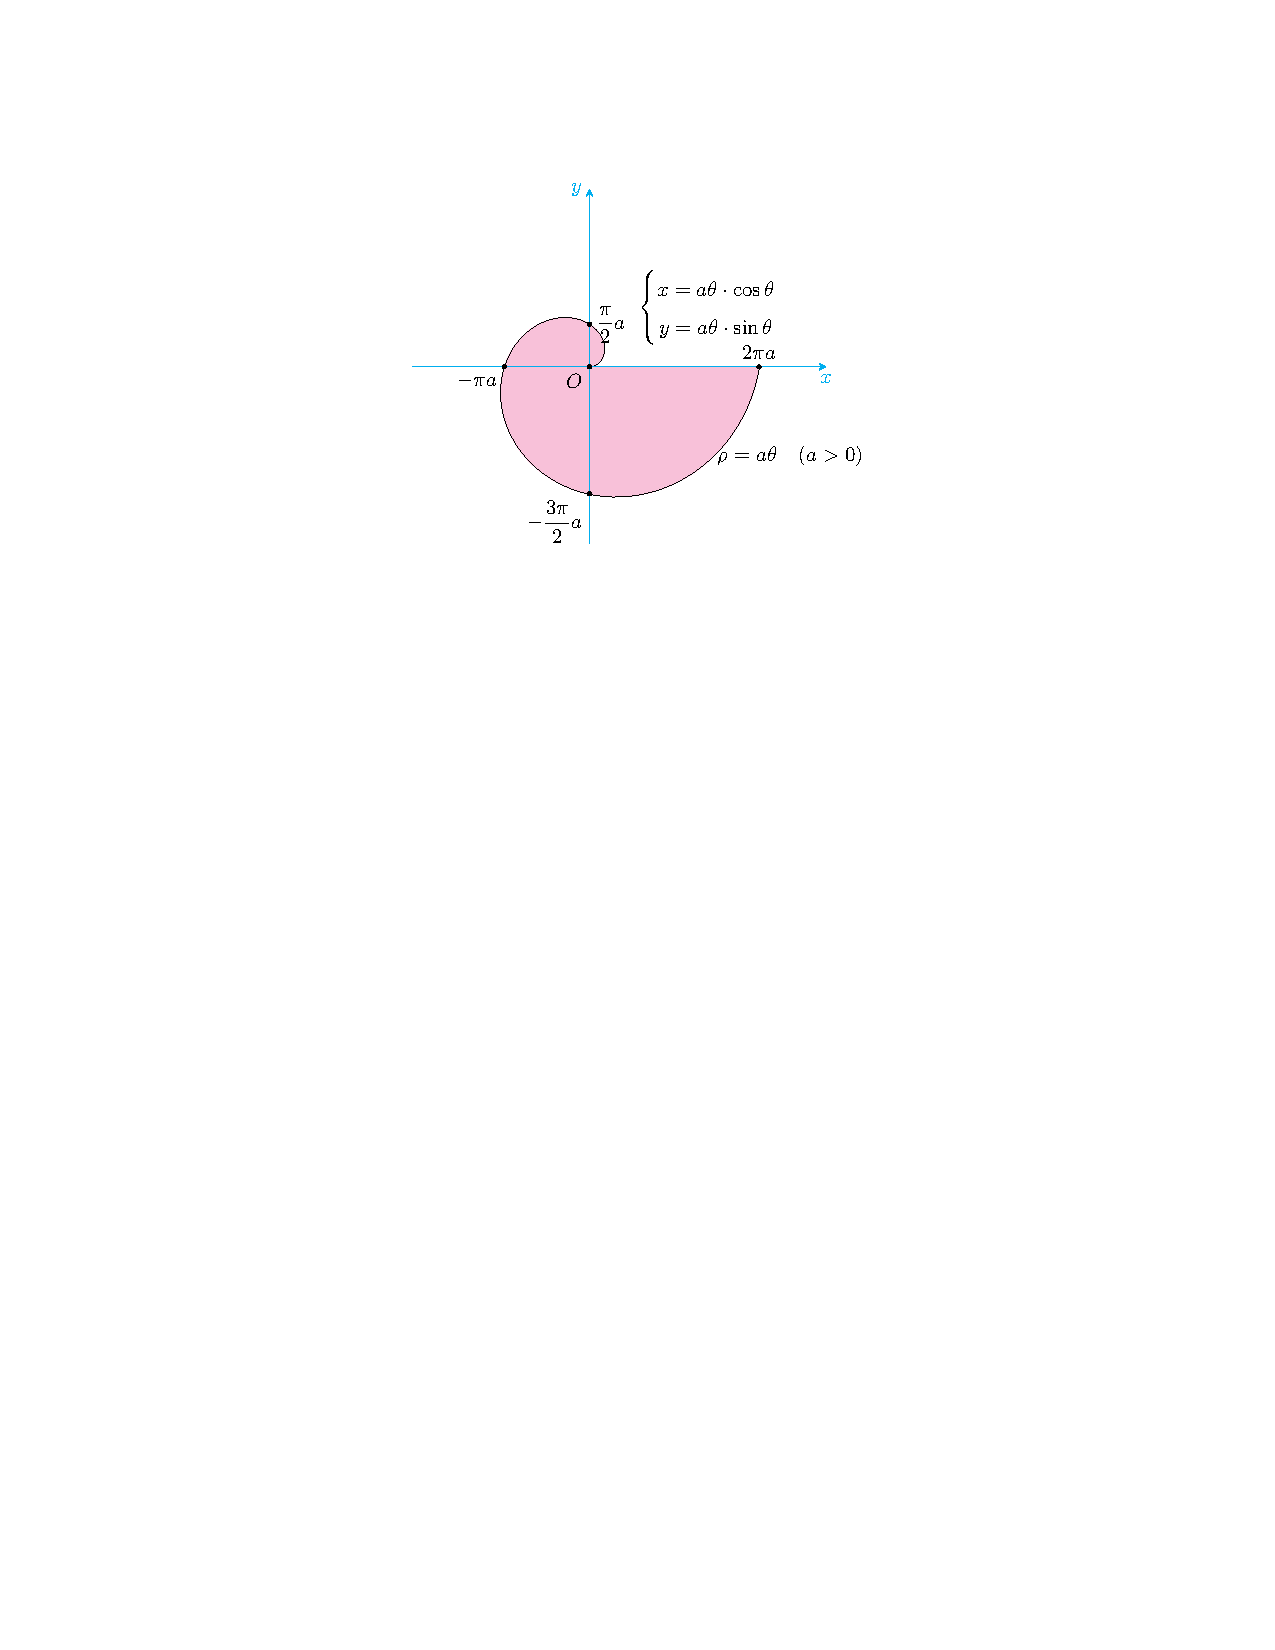
\includegraphics[scale=0.5]{figures/ArchimedesSpiral.pdf}
%     }\\
%     \subfigure[星形线]{
%         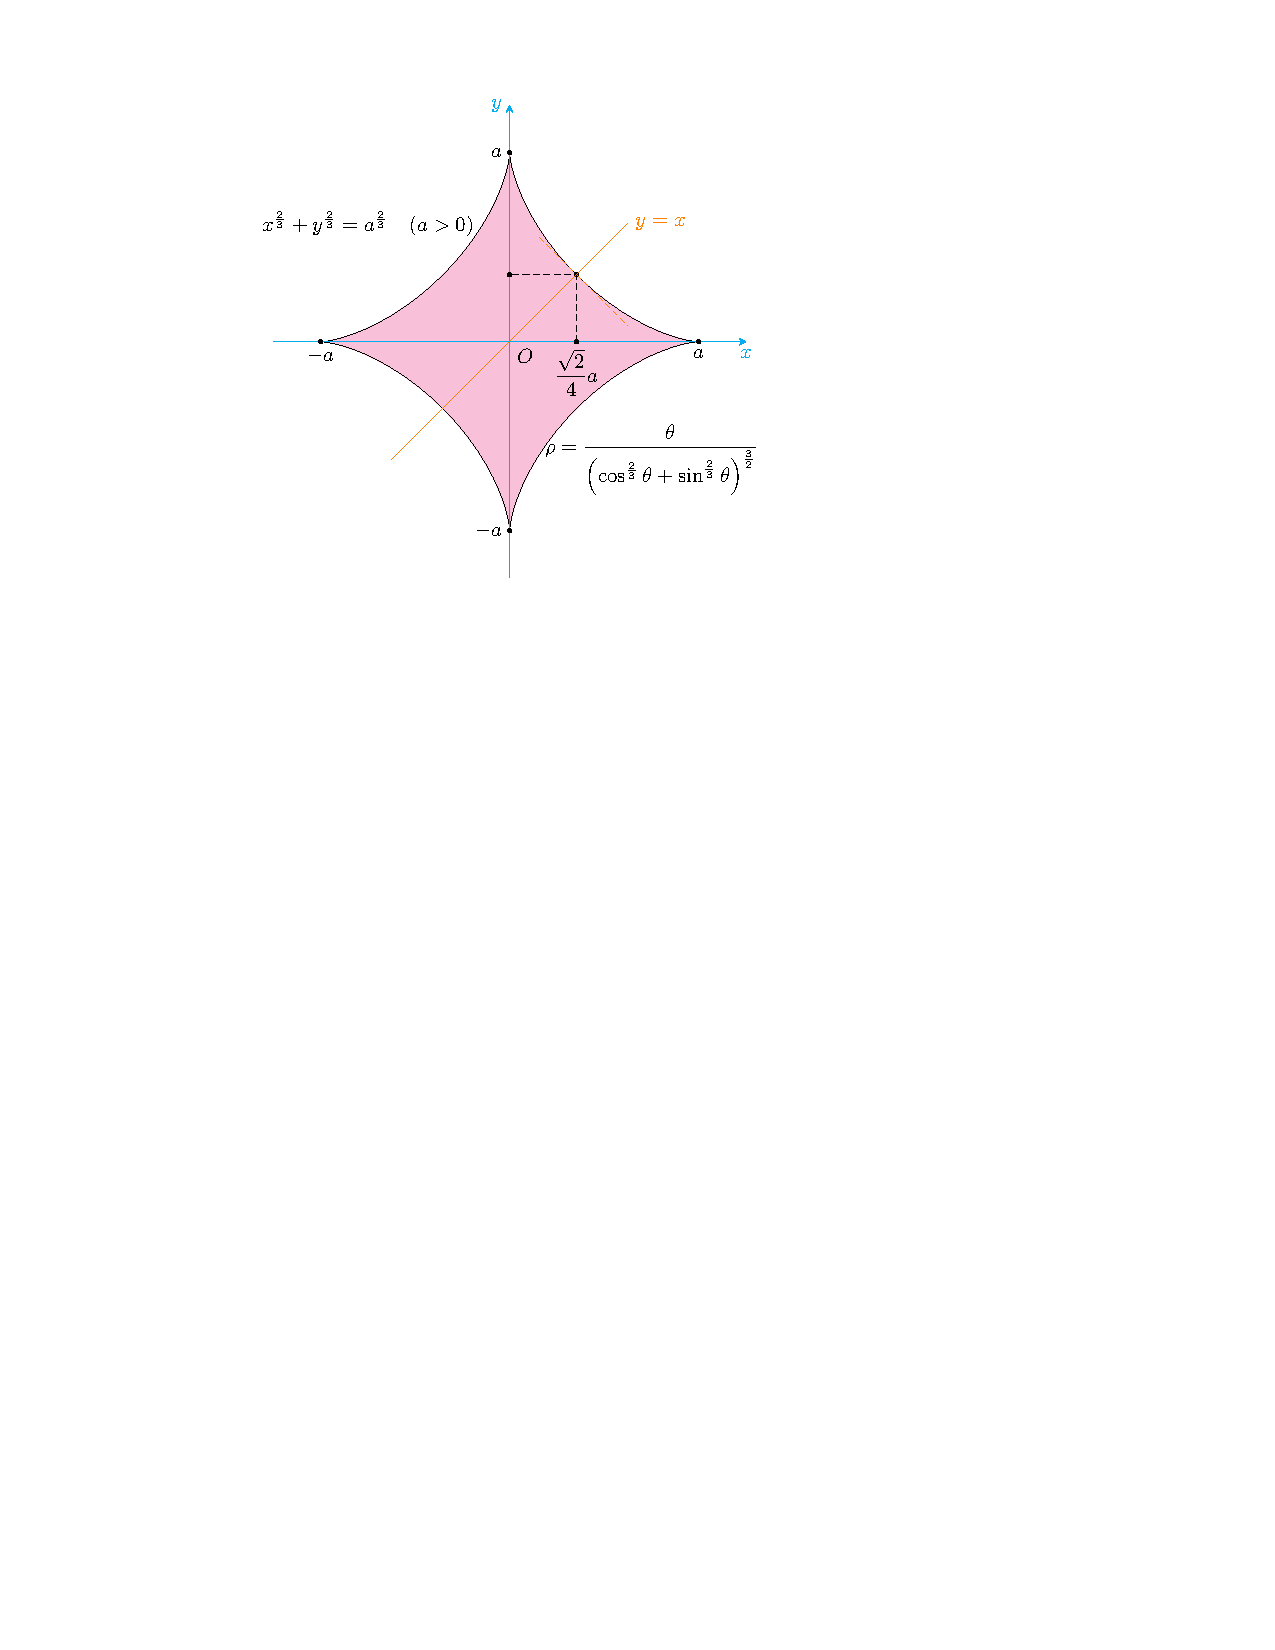
\includegraphics[scale=0.5]{figures/StarLine.pdf}
%     }
%     \subfigure[心形线]{
%         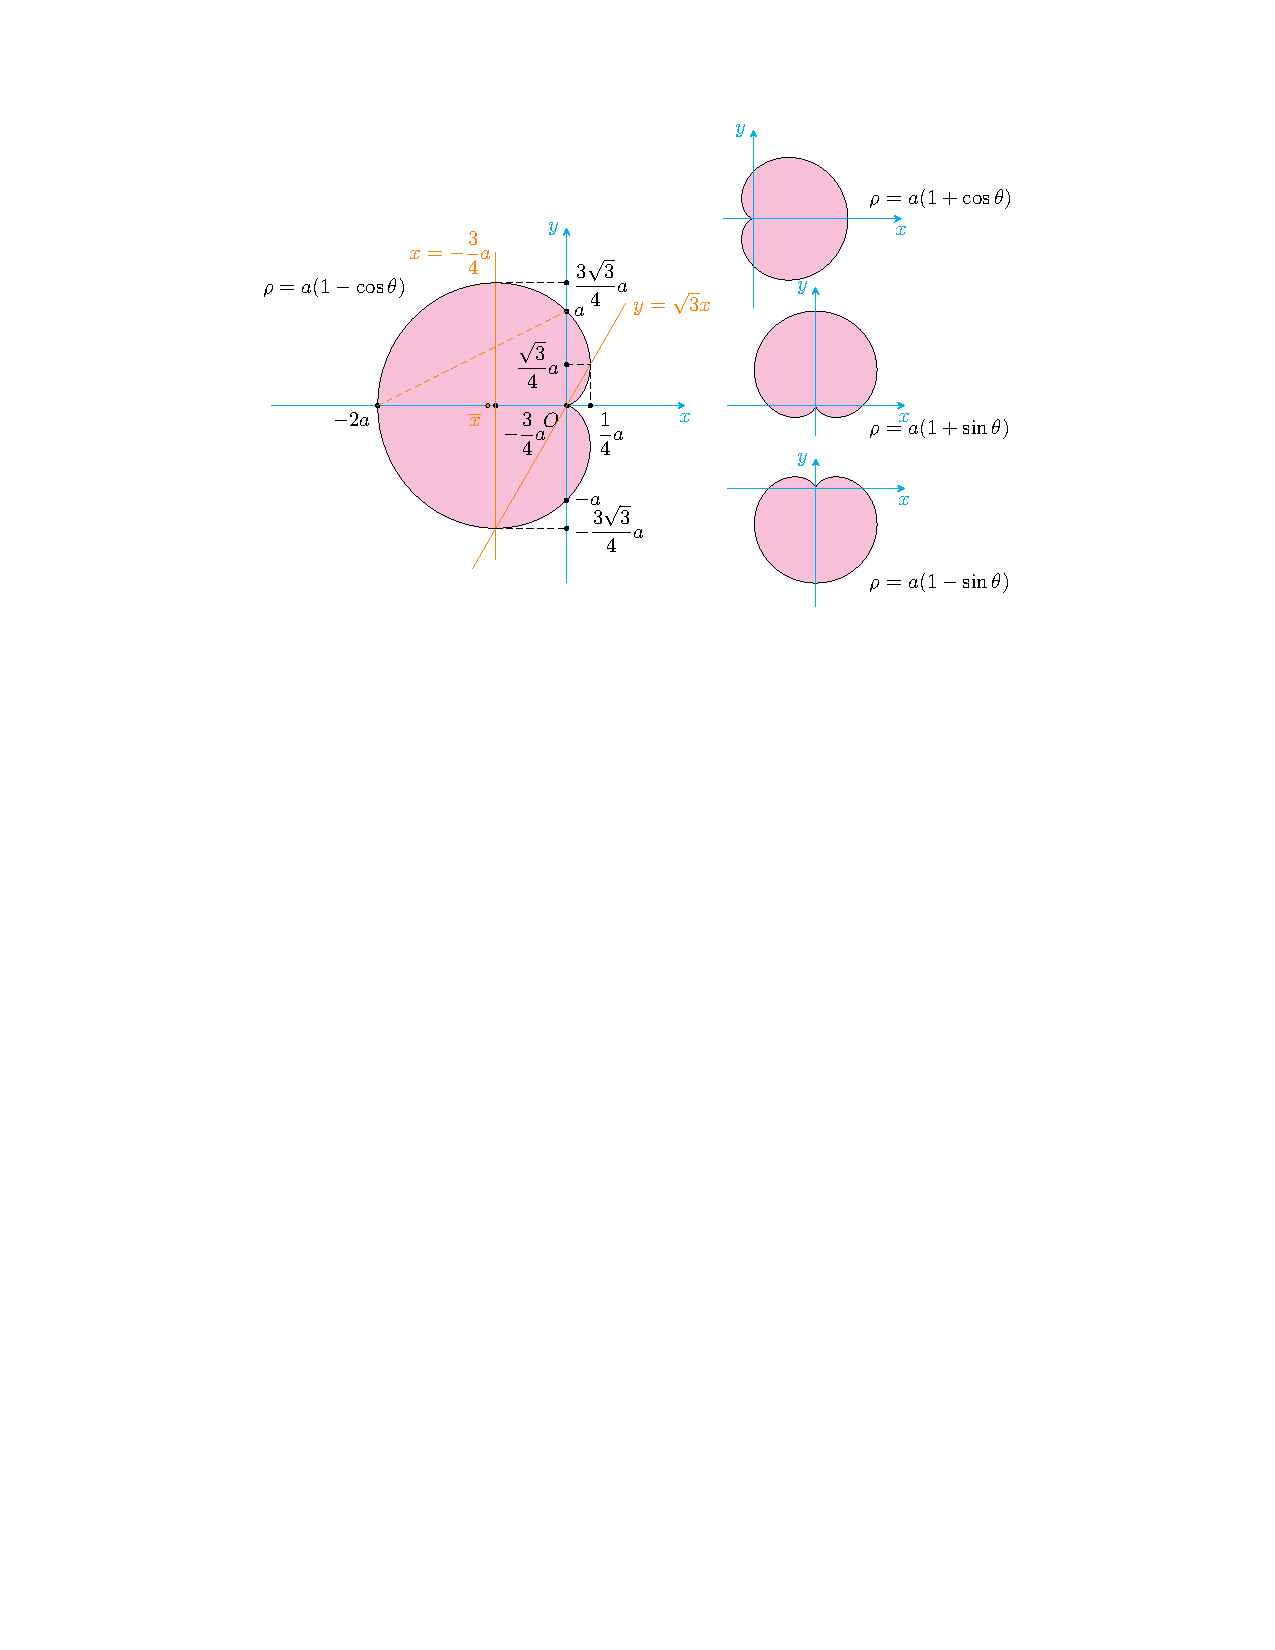
\includegraphics[scale=0.5]{figures/CardioidLine.pdf}
%     }\\
%     \subfigure[叶形线]{
%         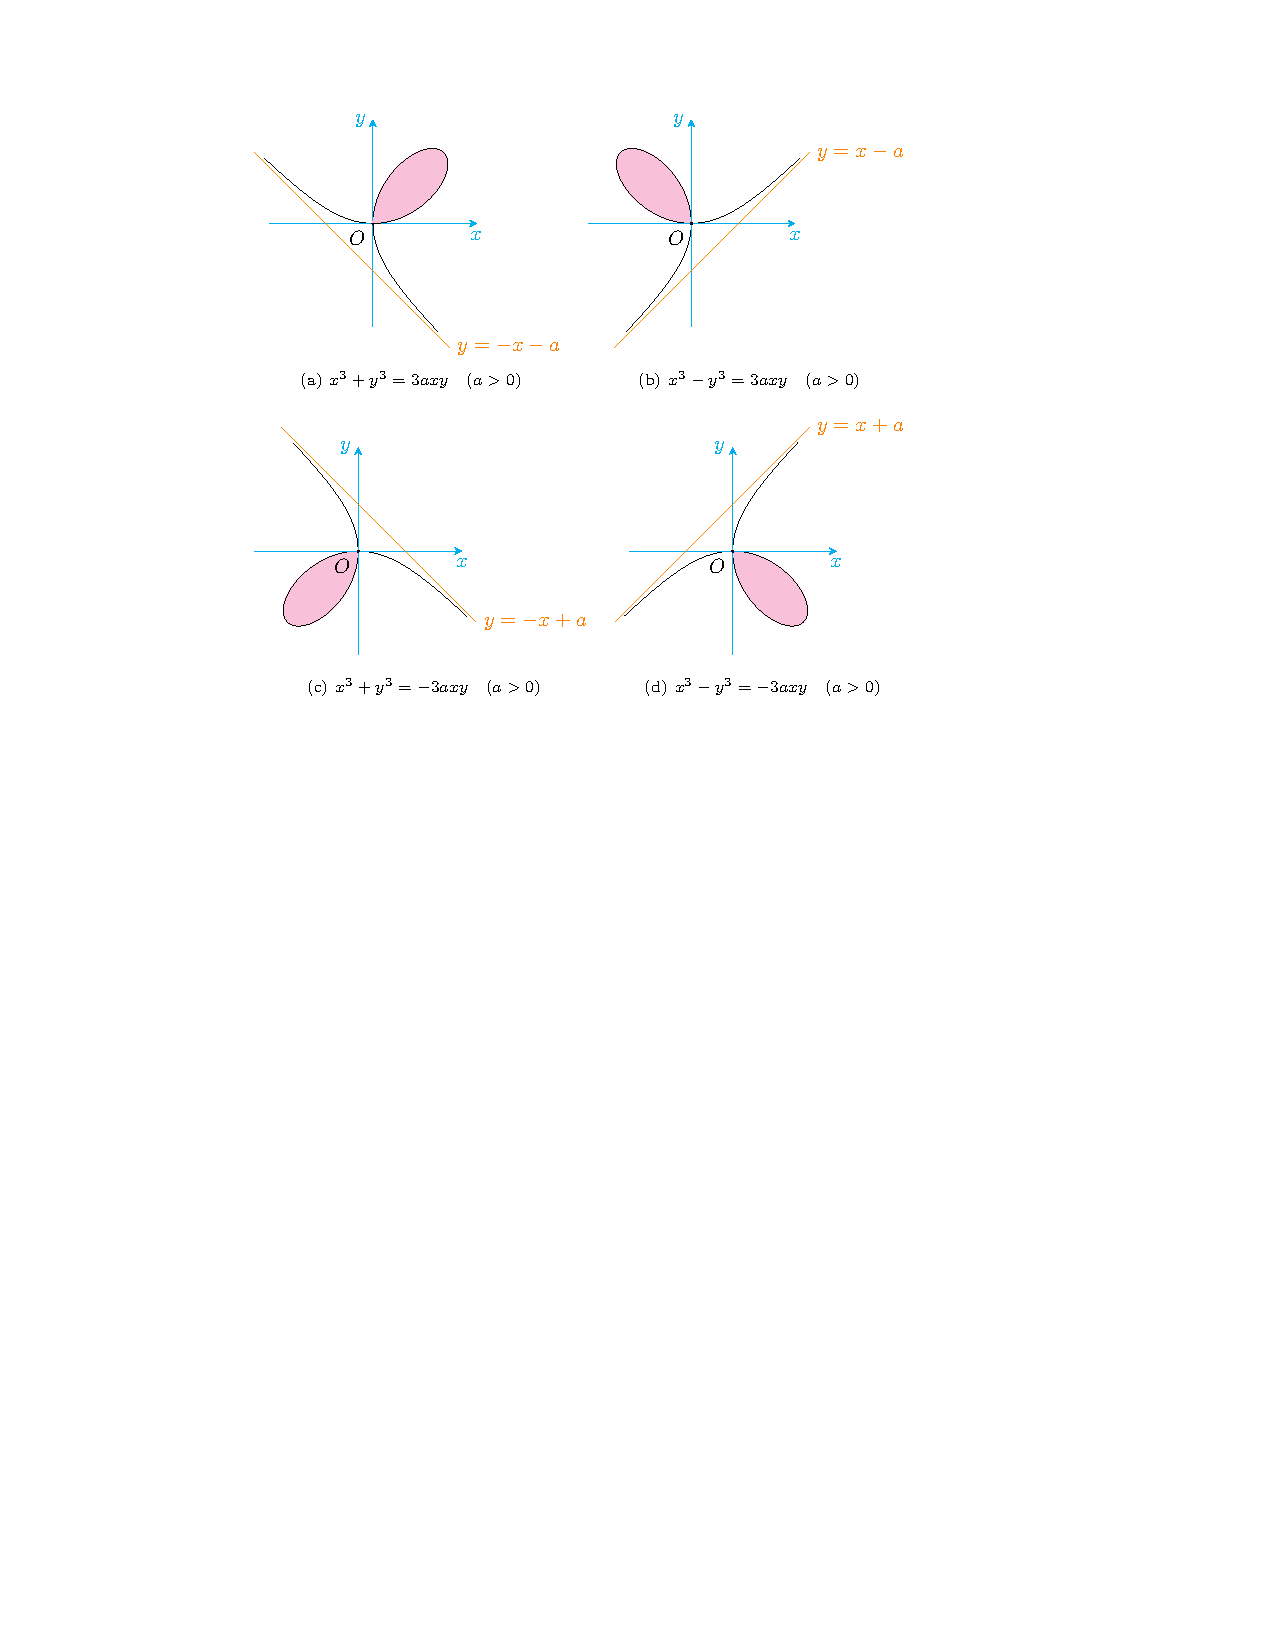
\includegraphics[scale=0.5]{figures/LeafLinear.pdf}
%     }
%     \subfigure[玫瑰线]{
%         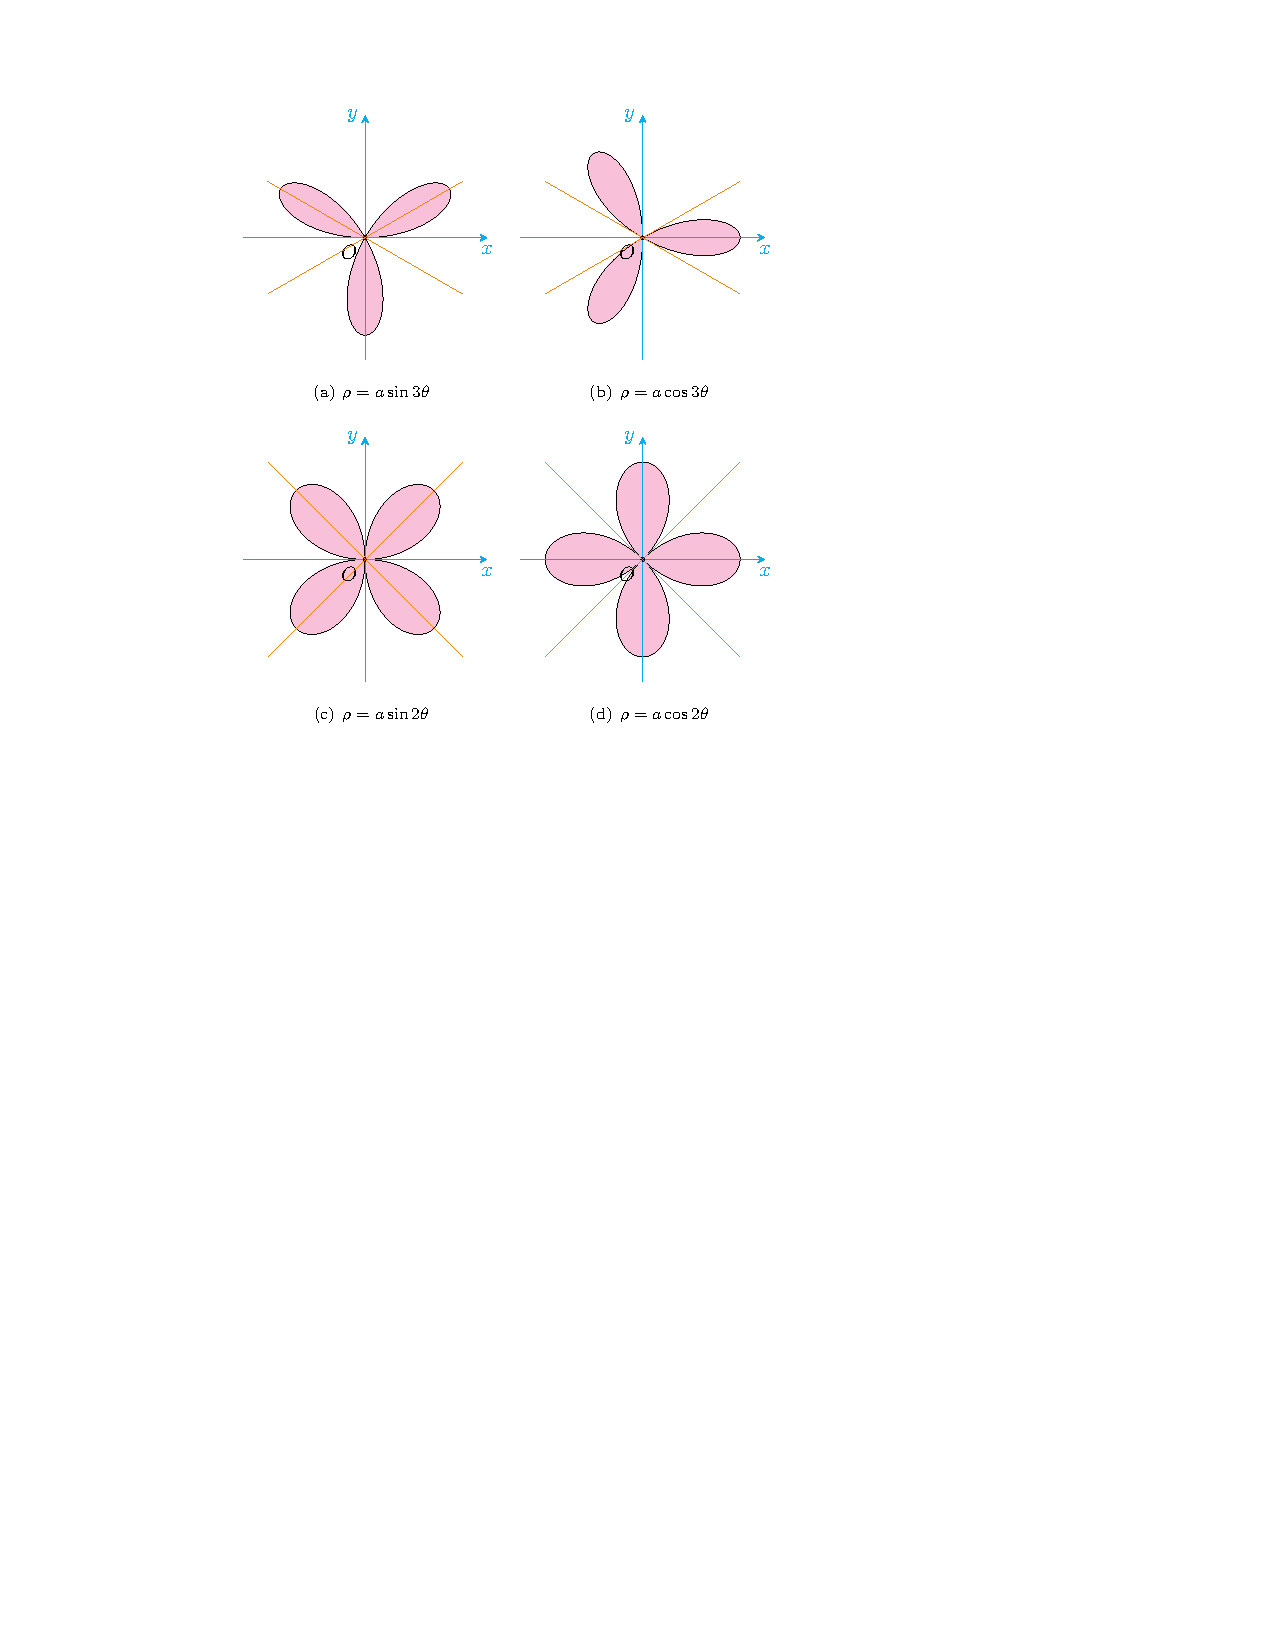
\includegraphics[scale=0.5]{figures/RoseLine.pdf}
%     }
%     \caption{常见的曲线及其对应方程}
% \end{figure}

% \subsection{向量值函数的导数与积分}